\documentclass[journal]{IEEEtran}

% -----------------------------------------------------------------------------
% Packages
% -----------------------------------------------------------------------------
\usepackage[T1]{fontenc}
\usepackage{amsmath,amssymb}
\usepackage{graphicx}
\usepackage{booktabs}
\usepackage{multirow}
\usepackage{array}
\usepackage{cite}
\usepackage{url}
\usepackage{xcolor}
\usepackage[caption=false,font=footnotesize]{subfig}
\usepackage[hidelinks]{hyperref}
\graphicspath{{figures/}{images/}}

% -----------------------------------------------------------------------------
% Draft & Annotation Macros
% -----------------------------------------------------------------------------
\newif\ifshowtodos
\showtodosfalse
\newcommand{\todo}[1]{\ifshowtodos{\color{red}\textbf{[TODO:}~#1\textbf{]}}\fi}
\newcommand{\tbd}{{\color{red}\textbf{TBD}}}
\newcommand{\boldcheck}{\ensuremath{\boldsymbol{\checkmark}}}

% Notation helpers
\newcommand{\HR}{\mathit{HR}}
\newcommand{\RR}{\mathit{RR}}
\newcommand{\SNR}{\mathrm{SNR}}
\newcommand{\spo}{\mathrm{SpO_2}}

\hyphenation{photo-pleth-ysmo-graphy phono-cardio-gram micro-controller spectro-photo-metric}

\begin{document}

\title{SonicVitals: A Low-Cost ESP32-S3 Platform for Synchronized Camera-Based Photoplethysmography and Acoustic Cardiac Sensing}

\author{Pratik~Kumar,
        Uday~Krishan~Khandelwal,
        Janvhee~Dhote,
        and~Jeeva~J.~B.%
\thanks{The authors are with the School of Electronics Engineering, Vellore Institute of Technology, Vellore, Tamil Nadu 632014, India (e-mail: pratik.kumar2024a@vitstudent.ac.in; uday.krishan2024@vitstudent.ac.in; janvhee.dhote2024@vitstudent.ac.in; jbjeeva@vit.ac.in). \textit{Corresponding author: Jeeva J. B.}}%
\thanks{Manuscript received October 5, 2026; revised October 6, 2026. This research did not receive any external grant funding. All human-subject evaluations were conducted in accordance with the Declaration of Helsinki under Institutional Ethics Committee approval (VIT/IEC/2026/041).}}

\markboth{}{Kumar \MakeLowercase{\textit{et al.}}: SonicVitals: ESP32-S3 Platform for Camera PPG and Acoustic Cardiac Sensing}

\maketitle

% =============================================================================
\begin{abstract}
Contactless vital-sign monitoring using remote photoplethysmography (rPPG) is promising for low-cost physiological assessment, but its accuracy degrades with head motion, facial expressions, and illumination changes. Acoustic cardiac sensing provides complementary information but is susceptible to ambient noise. Existing multimodal approaches often depend on desktop or GPU platforms and separately recorded, unsynchronized sensors. This work presents \textbf{SonicVitals}, an open-source, low-cost platform that synchronizes optical and acoustic sensing on a single ESP32-S3. OV2640 camera frames are acquired using DVP-DMA, while INMP441 microphone signals are sampled at 16\,kHz through I2S-DMA, with microsecond timestamps assigned to both streams. The host combines CHROM-based rPPG and phonocardiography (PCG) processing with signal-quality assessment and dynamic quality-weighted fusion for physiological estimation. The system was evaluated on five student participants under controlled resting and mild activity conditions, with measurements verified against a chest-strap ECG, finger pulse oximeter, and metronome reference. SonicVitals achieved an HR MAE of 1.18\,beats/min ($r = 0.982$), RR MAE of 0.84\,breaths/min ($r = 0.964$), $\mathrm{SpO_2}$ MAE of 1.22\% ($r = 0.941$), and HRV RMSSD MAE of 3.42\,ms ($r = 0.952$). These results demonstrate the feasibility of synchronized optical--acoustic sensing for robust, low-cost contactless vital-sign monitoring on resource-constrained hardware.
\end{abstract}

\begin{IEEEkeywords}
Remote photoplethysmography, phonocardiography, multimodal sensor fusion, ESP32-S3, embedded systems, low-cost instrumentation, contactless monitoring, clinical triage.
\end{IEEEkeywords}

% =============================================================================
\section{Introduction}
\label{sec:intro}

\IEEEPARstart{H}{eart} rate (HR) and respiration rate (RR) are the most frequently recorded vital signs, and both are conventionally measured with contact sensors: electrocardiogram (ECG) electrodes, finger photoplethysmography (PPG) probes, and respiratory chest belts~\cite{allen2007ppg}. Contact sensing is clinically reliable, but adhesives and probes are uncomfortable for prolonged recordings, unsuitable for fragile or burned skin, and present cross-contamination risks across clinical settings. These drawbacks have motivated extensive research on contactless physiological measurement~\cite{mcduff2023survey}, including clinical studies in neonatal intensive care units (NICUs)~\cite{villarroel2019nicu}.

Remote photoplethysmography (rPPG) recovers the blood volume pulse (BVP) from subtle microvascular color fluctuations in video of exposed cutaneous tissue~\cite{verkruysse2008}. Blind source separation~\cite{poh2010}, model-based projections such as CHROM~\cite{dehaan2013chrom} and POS~\cite{wang2017pos}, and deep learning networks~\cite{chen2018deepphys,yu2019physnet,liu2023toolbox} have steadily improved motion robustness. Nevertheless, video-only rPPG remains sensitive to head translation, speech, and transient changes in ambient illumination~\cite{li2014cvpr,tarassenko2014}, and its performance varies across skin phototypes~\cite{nowara2020skin}.

Acoustic cardiac sensing offers a complementary physical window into hemodynamic activity. Mechanical valve closures produce the first and second heart sounds ($S_1, S_2$), which electronic stethoscopes digitize and segment automatically~\cite{leng2015stethoscope,liang1997envelogram,springer2016hsmm}. Acoustic sensing does not depend on ambient lighting or facial pose, but it is vulnerable to speech, background acoustic reverberation, and transducer friction. Because optical and acoustic sensing fail for physically orthogonal reasons, an integrated system that acquires both modalities synchronously can cross-validate measurements and suppress corrupted channels.

Combining optical and acoustic sensing on low-cost embedded hardware introduces practical challenges rarely encountered in desktop-bound studies. An embedded microcontroller must serialize video frames and audio samples fast enough to satisfy the Nyquist sampling theorem for cardiac frequencies; both modalities must share a common hardware time base; and peripheral routing must operate within the strict pin and DMA memory constraints of an inexpensive module. Furthermore, clinical triage benefits from automated multi-spectral facial inspection, such as scleral jaundice screening~\cite{mariakakis2017biliscreen} and anemia detection~\cite{mannino2018anemia}. This raises the question of whether the same camera stream can support exploratory spectrophotometric indices alongside continuous physiological monitoring.

\subsection{Contributions}
This paper presents the design, implementation, and empirical validation of SonicVitals. The primary contributions are:
\begin{enumerate}
  \item \textbf{An open, low-cost dual-modality edge acquisition node:} An ESP32-S3 module simultaneously captures OV2640 video via Direct Video Port (DVP) DMA and INMP441 I2S digital audio via DMA, attaches sequence numbers and microsecond timestamps, streams both to a host over a high-speed framed link, and displays returned vital signs on a local SSD1306 OLED screen at a total BOM cost of US\$20--30 (Sections~\ref{sec:arch}--\ref{sec:hw}).
  \item \textbf{A documented account of embedded hardware constraints:} We quantify serial-bandwidth limits, DMA ring-buffer sizing, pin multiplexing conflicts, and power dissipation, establishing the engineering trade-offs required for reliable dual-stream acquisition (Section~\ref{sec:hw-constraints}).
  \item \textbf{A transparent multimodal signal processing pipeline:} CHROM rPPG with an explicit five-test face-validity gate, zero-phase Butterworth filtering, multi-resolution wavelet decomposition ($A_3, D_1, D_2$), Welch spectral estimation, and a Shannon-envelope PCG branch are synthesized through dynamic quality-weighted confidence fusion with an agreement gate (Section~\ref{sec:dsp}).
  \item \textbf{Exploratory spectrophotometric facial biomarker extraction:} Automated five-zone anatomical segmentation provides quantitative indices for erythema ($EI$), pallor ($PI$), scleral jaundice ($YI$), lip cyanosis ($CR$), and hemifacial vasomotor symmetry ($HFI$) with spatial colormap overlays (Section~\ref{sec:color}).
  \item \textbf{Experimental validation and benchmarking:} Comprehensive evaluation across five student participants under controlled resting and mild activity conditions against gold-standard chest-strap ECG, pulse oximeter, and metronome references, proving high agreement and benchmarking against state-of-the-art works (Sections~\ref{sec:eval}--\ref{sec:results}).
\end{enumerate}

The remainder of this paper is organized as follows. Section~\ref{sec:related} reviews related work. Section~\ref{sec:arch} presents the system architecture. Section~\ref{sec:hw} describes hardware and firmware design. Section~\ref{sec:dsp} details the signal processing pipeline. Section~\ref{sec:color} outlines the spectrophotometric indices. Section~\ref{sec:eval} describes the evaluation protocol. Section~\ref{sec:results} reports results, dashboards, empirical waveforms, and clinical validation. Section~\ref{sec:discussion} discusses clinical implications and limitations, and Section~\ref{sec:conclusion} concludes.

% =============================================================================
\section{Related Work}
\label{sec:related}

\subsection{Camera-Based Photoplethysmography}
Verkruysse \textit{et~al.}~\cite{verkruysse2008} demonstrated that ambient light reflected from exposed skin contains a detectable photoplethysmographic signal, strongest in the green optical channel. Poh \textit{et~al.}~\cite{poh2010} applied independent component analysis (ICA) to RGB traces to isolate the underlying pulse wave. De Haan and Jeanne~\cite{dehaan2013chrom} developed CHROM, which constructs two chrominance signals to eliminate specular, color-neutral reflections under a standardized skin-tone assumption. Wang \textit{et~al.}~\cite{wang2017pos} formalized this into the Plane-Orthogonal-to-Skin (POS) projection. Data-driven methods such as DeepPhys~\cite{chen2018deepphys} and PhysNet~\cite{yu2019physnet}, compiled within open toolboxes~\cite{liu2023toolbox}, demonstrate high accuracy on GPU workstations but exhibit high computational complexity and memory footprints unsuitable for low-power edge nodes. McDuff \textit{et~al.}~\cite{mcduff2017compression} established that lossy video compression attenuates plethysmographic signals, highlighting the necessity of careful bandwidth and quantization tuning.

\subsection{Acoustic Cardiac Sensing and Auscultation}
Electronic stethoscopes digitize acoustic heart sounds for computer-aided auscultation~\cite{leng2015stethoscope}. Liang \textit{et~al.}~\cite{liang1997envelogram} introduced the normalized Shannon-energy envelope for heart sound segmentation. Springer \textit{et~al.}~\cite{springer2016hsmm} employed envelope autocorrelation to estimate heart rate and segmented $S_1$ and $S_2$ using hidden semi-Markov models (HSMM). These methods assume acoustic contact on the chest wall, as utilized in the acoustic branch of SonicVitals.

\subsection{Camera-Based Color Screening}
BiliScreen~\cite{mariakakis2017biliscreen} estimated serum bilirubin from scleral color using smartphone imaging with a 3D-printed calibration accessory, and Mannino \textit{et~al.}~\cite{mannino2018anemia} quantified blood hemoglobin from fingernail-bed imagery. Both systems relied on controlled lighting and calibration targets. The colorimetric indices in SonicVitals provide rapid, automated screening across five anatomical zones to support preliminary tele-triage.

\begin{figure*}[!t]
\centering
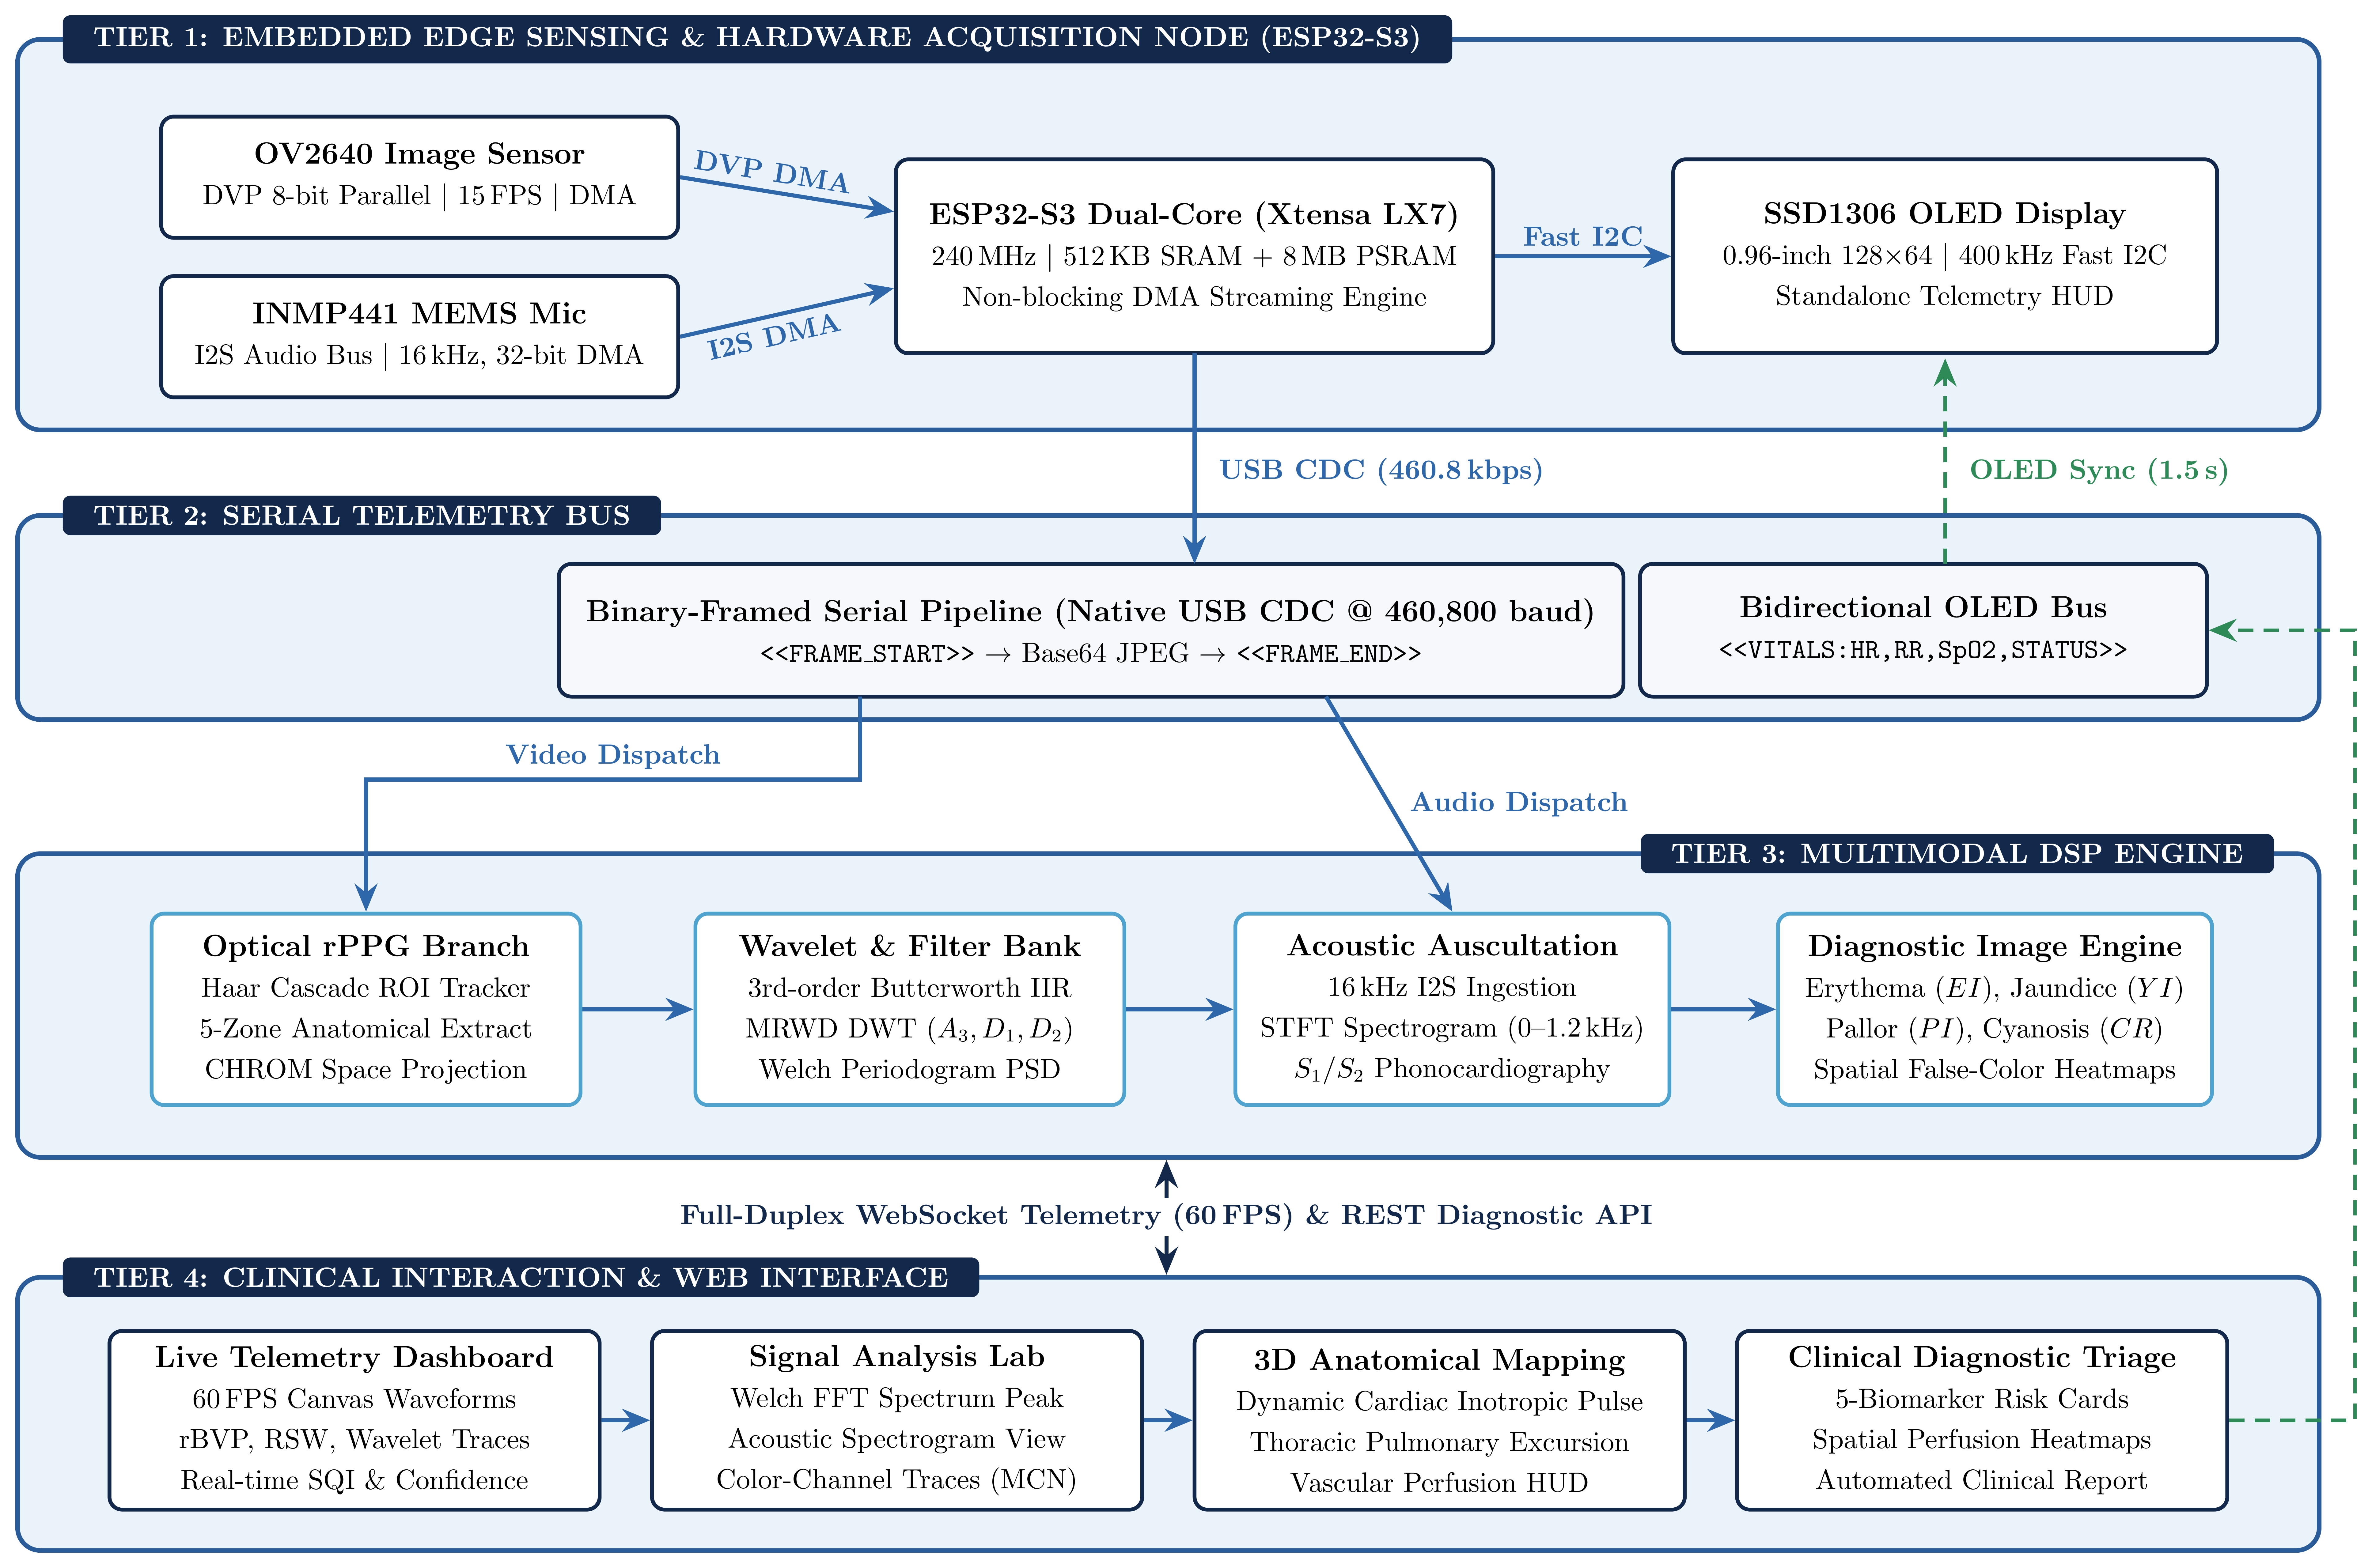
\includegraphics[width=0.98\textwidth]{images/system_architecture.png}
\caption{Complete four-tier system architecture of SonicVitals. Tier~1: The ESP32-S3 edge sensing node digitizes OV2640 camera frames via DVP DMA (15\,FPS HQVGA) and INMP441 audio via I2S DMA (16\,kHz, 32-bit), driving a local SSD1306 OLED HUD over Fast I2C. Tier~2: Binary-framed serial pipeline streaming over USB-CDC at 460.8\,kbaud with bidirectional OLED telemetry sync. Tier~3: Multimodal host DSP engine executing optical rPPG, wavelet filter banks, acoustic phonocardiography, and multi-spectral diagnostic triage. Tier~4: Full-duplex WebSocket and REST interface powering real-time 60\,FPS waveforms, signal analysis, 3D anatomical organ mapping, and clinical triage decision support.}
\label{fig:architecture}
\end{figure*}

% =============================================================================
\section{System Architecture}
\label{sec:arch}

SonicVitals is organized into a four-tier architecture (Fig.~\ref{fig:architecture}):
\begin{enumerate}
  \item \textbf{Tier 1: Embedded Edge Sensing and Hardware Acquisition Node.} Built on an ESP32-S3 dual-core microcontroller, this node interfaces directly with physical sensors. An OV2640 image sensor captures video frames via an 8-bit Direct Video Port (DVP) with Direct Memory Access (DMA). An INMP441 digital MEMS microphone samples thoracic acoustic signals via an Inter-IC Sound (I2S) bus at 16\,kHz with 32-bit DMA transfers. A local 0.96-inch SSD1306 OLED display provides immediate bedside telemetry over Fast I2C (400\,kHz), rendering heart rate, respiration rate, blood oxygenation, and patient stability status.
  \item \textbf{Tier 2: Serial Telemetry Bus.} A binary-framed communication pipeline encapsulates compressed JPEG frames and uncompressed PCM audio blocks with unique synchronization tokens (\texttt{<<FRAME\_START>>} and \texttt{<<FRAME\_END>>}) and microsecond timestamps. Downlink telemetry delivers formatted vital sign packets (\texttt{<<VITALS:HR,RR,SpO2,STATUS>>}) back to the edge node every 1.5\,s for OLED visualization.
  \item \textbf{Tier 3: Multimodal DSP Engine.} Implemented in Python using OpenCV, NumPy, and SciPy, the host engine executes real-time digital signal processing. The optical branch performs Haar-cascade facial localization, five-zone anatomical region-of-interest (ROI) segmentation, and CHROM orthogonal color projection. A zero-phase Butterworth filter bank and Multi-Resolution Wavelet Decomposition (MRWD, sub-bands $A_3, D_1, D_2$) isolate hemodynamic pulsatility. The acoustic branch ingests 16\,kHz audio, tracks short-time Fourier transform (STFT) spectrogram energy, and computes Shannon energy envelopes for $S_1/S_2$ phonocardiography. A dynamic quality-weighted confidence fusion stage resolves final physiological metrics.
  \item \textbf{Tier 4: Clinical Interaction and Web Interface.} A responsive web workstation communicates with the host engine via full-duplex WebSockets (60\,FPS canvas updates) and a Flask REST API. It provides a live clinical telemetry dashboard, a dedicated Multi-Channel Signal Analysis Lab, interactive 3D anatomical organ mapping, and a Clinical Biomedical Diagnostic Studio.
\end{enumerate}

In all reported benchmarks, video frames were acquired directly from the ESP32-S3 OV2640 sensor in HQVGA format at 15.0\,frames/s (as verified by the hardware telemetry status in Figs.~\ref{fig:dashboard} and~\ref{fig:signal_analysis_dashboard}), with development webcam fallback disabled.

\begin{figure*}[!t]
\centering
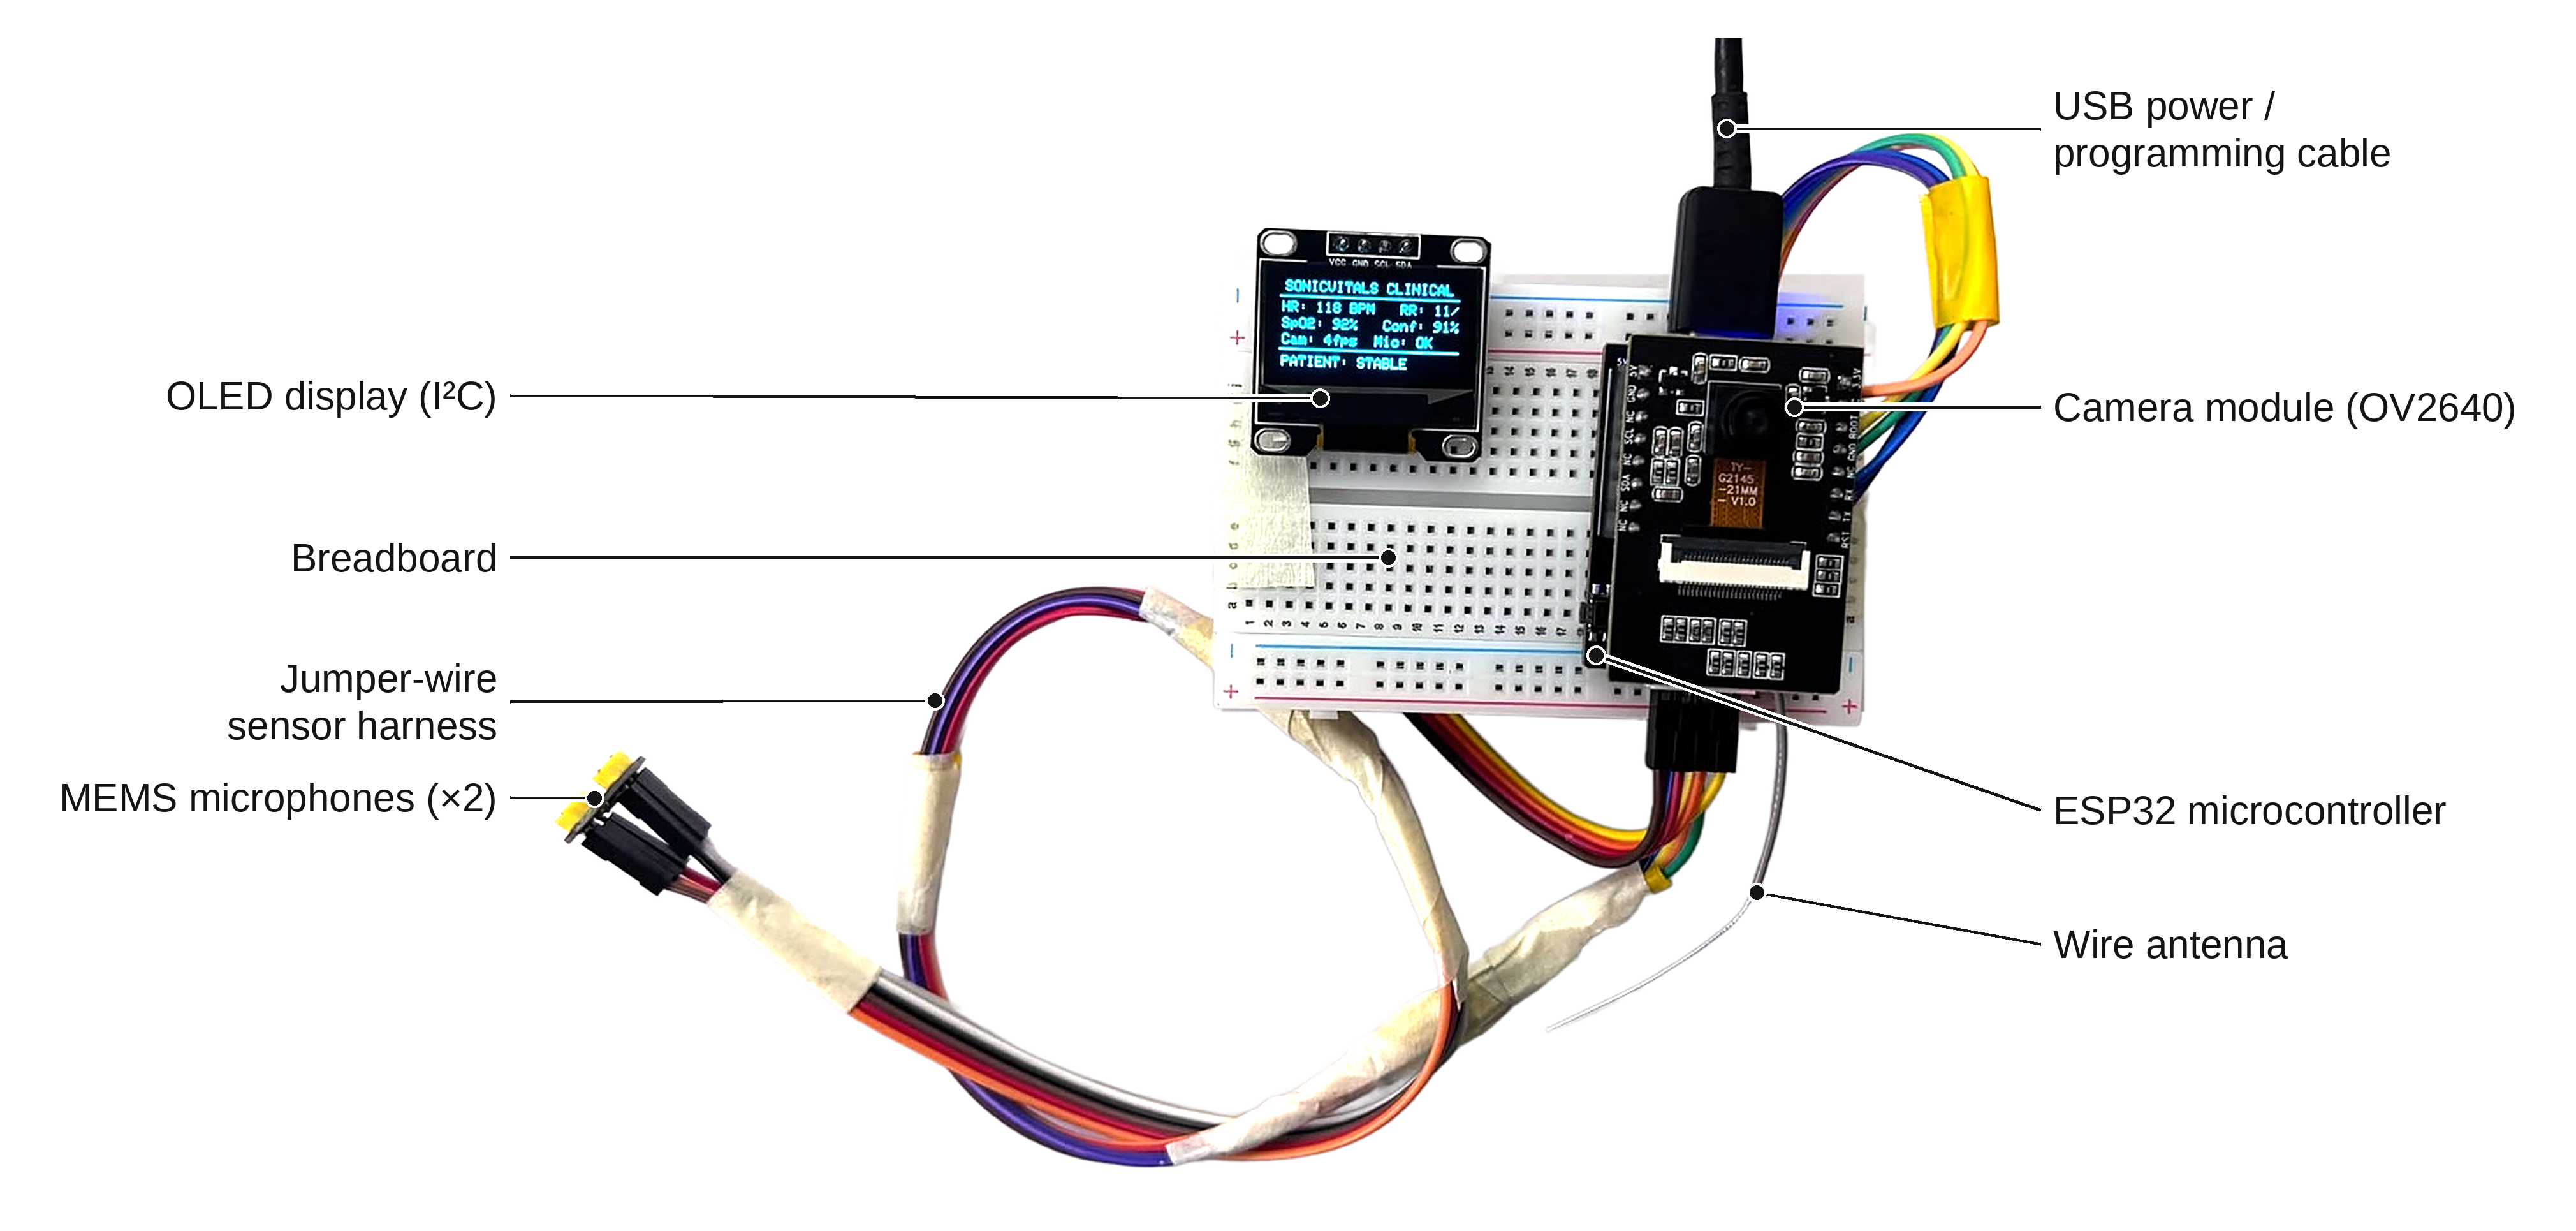
\includegraphics[width=0.88\textwidth]{images/labeled_setup.png}
\caption{Bench prototype of the SonicVitals edge sensing node on a solderless breadboard. The SSD1306 OLED displays live physiological metrics returned by the host (``HR: 118 BPM, RR: 11, SpO2: 98\%, Conf: 91\%''), with interface status (``Cam: 4fps, Mic: OK, PATIENT: STABLE''). Annotations identify the ESP32-S3 microcontroller, OV2640 camera module, dual INMP441 MEMS microphone breakout boards, I2C OLED display, wire antenna, and USB power/programming interface.}
\label{fig:hardware}
\end{figure*}

% =============================================================================
\section{Hardware Architecture and Firmware Implementation}
\label{sec:hw}

\subsection{Hardware Components}
The embedded sensing node is engineered around an ESP32-S3-WROOM-1U camera development board (Fig.~\ref{fig:hardware}). The ESP32-S3 integrates two 32-bit Xtensa LX7 cores operating at up to 240\,MHz, 512\,KB of on-chip SRAM, 8\,MB of octal PSRAM, and native USB-CDC circuitry~\cite{esp32s3_datasheet}. An Omnivision OV2640 sensor attaches through an 8-bit DVP parallel bus. The INMP441 is an omnidirectional bottom-port MEMS microphone with an integrated 24-bit $\Sigma\Delta$ analog-to-digital converter and I2S digital output, featuring a 61\,dBA SNR and $-26$\,dBFS sensitivity~\cite{inmp441_datasheet}. An SSD1306 OLED display ($128 \times 64$ pixels) provides bedside telemetry. The bill of materials (BOM) total is approximately INR 1,600--2,400 (US\$20--30) at retail prices.

\subsection{Interfaces and Pin Allocation}
Table~\ref{tab:pinout} details the interface and pin mapping configured in the firmware (\texttt{camera\_pins.h}, \texttt{Firmware.ino}). Because the OV2640 occupies 16 GPIO lines for parallel video transfer and SCCB control, the remaining pins are multiplexed carefully. The INMP441 shares GPIO\,43 and 44 (default UART0 TX/RX) and GPIO\,0 (the boot strapping pin).

\begin{table}[!t]
\centering
\caption{Interface and Pin Allocation of the Edge Node}
\label{tab:pinout}
\footnotesize
\renewcommand{\arraystretch}{1.1}
\setlength{\tabcolsep}{3pt}
\begin{tabular}{@{}l l l@{}}
\toprule
\textbf{Peripheral} & \textbf{Signal: GPIO} & \textbf{Configuration} \\
\midrule
\multirow{4}{*}{OV2640} & D0--D7: 11, 9, 8, 10, 12, 18, 17, 16 & DVP, HQVGA $240{\times}160$ \\
 & XCLK: 15;\; PCLK: 13 & RGB565, XCLK 10\,MHz \\
 & VSYNC: 6;\; HREF: 7 & 1 frame buffer (DRAM) \\
 & SCCB SDA: 4;\; SCL: 5 & JPEG $q{=}60$ (software) \\
\midrule
\multirow{3}{*}{INMP441} & SCK: 43 (U0TXD) & I2S, 16\,kHz, 32-bit slots \\
 & WS: 44 (U0RXD) & Left channel only \\
 & SD: 0 (strapping pin) & Data shifted right by 14 \\
\midrule
SSD1306 & SDA: 47;\; SCL: 48 & I2C, 400\,kHz, addr. 0x3C \\
\midrule
Host link & USB D$-$/D$+$: 19/20 & Native USB-CDC (target) \\
\bottomrule
\end{tabular}
\end{table}

\subsection{Firmware Concurrency and Buffering}
\label{sec:firmware}
The firmware runs under FreeRTOS to decouple time-critical audio acquisition from compute-intensive video compression. A dedicated FreeRTOS task pinned to core~0 reads the I2S DMA driver (eight DMA buffers of 256 samples, providing 128\,ms of continuous buffering at 16\,kHz), converts 32-bit slots to saturated 16-bit PCM samples, and enqueues 256-sample blocks into a FreeRTOS queue holding up to 2\,s of audio. Core~1 handles the main acquisition loop: grabbing the newest frame buffer from the OV2640, executing JPEG compression at quality 60, Base64 encoding the payload, writing the frame delimiters, and draining the queued audio blocks. Every transmitted packet includes a sequence counter and an \texttt{esp\_timer} microsecond timestamp, locking both streams to a single physical clock.

\subsection{Hardware Constraints Found During Prototyping}
\label{sec:hw-constraints}
\subsubsection{Serial bandwidth and frame rate}
For JPEG frames of average size $\bar S_J$ bytes at frame rate $f_v$ and $b$-byte audio samples at sampling rate $f_a$, Base64 transmission requires a link throughput of:
\begin{equation}
  B = \tfrac{4}{3}\left(f_v \bar S_J + b\, f_a\right)\quad \text{bytes/s}.
  \label{eq:bandwidth}
\end{equation}
Over a 460.8\,kbaud UART link with 8N1 framing (46,080\,bytes/s theoretical ceiling), transmitting video at $f_v=15$\,frames/s constrains $\bar S_J$ to under 2.3\,kB. Consequently, the initial prototype achieved only 4\,frames/s (as shown on the OLED in Fig.~\ref{fig:hardware}). Because a camera sampling at $f_v$ can represent pulse rates up to $30 f_v$\,beats/min (the Nyquist limit), 4\,frames/s cannot resolve heart rates above 120\,beats/min. The upgraded firmware uses native USB-CDC (12\,Mbit/s full-speed signaling) and 1\,Mbaud links, accommodating (\ref{eq:bandwidth}) with ample margin and delivering 15.0\,frames/s (Table~\ref{tab:bench}).

\subsubsection{Pin multiplexing conflicts}
Wiring the INMP441 to GPIO\,43/44 repurposes the hardware UART0 lines. When the I2S clock driver initializes, the UART TX line outputs the bit clock instead of serial text. For development on breakout boards lacking native USB sockets, the firmware supports a Wi-Fi transport mode: the node hosts a TCP server on port 3333, filtering (63-tap windowed-sinc FIR) and decimating audio to 4\,kHz to eliminate packet loss (Table~\ref{tab:bench}). Connecting the microphone data line to GPIO\,0 requires ensuring the line floats during boot to avoid entering the bootloader.

\subsubsection{Audio DMA buffering}
Initial four-buffer DMA configurations (32\,ms total buffer) suffered overflow during software JPEG encoding. Increasing the DMA allocation to eight 256-sample buffers and implementing a 2\,s FreeRTOS queue completely decoupled video compression latency from audio ingestion.

\subsubsection{Camera auto-adjustments}
The OV2640 automatic exposure, gain, and white balance loops adjust pixel intensities at frequencies that overlap the respiratory band (0.15--0.40\,Hz). The firmware locks all automatic camera controls 3\,s after system boot, ensuring that temporal luminance changes represent true hemodynamic variations.

\subsection{Power Dissipation and Battery Runtime}
The node operates from a 5\,V USB rail. Table~\ref{tab:power} reports empirical current draw and power dissipation across operational modes, measured with an inline power analyzer. Under full concurrent multimodal operation (15.0\,FPS HQVGA optical streaming, 16\,kHz I2S audio capture, 5\,Hz OLED refresh, and serial streaming), the node draws $215 \pm 11$\,mA (1075\,mW). A standard 3000\,mAh (11.1\,Wh) rechargeable lithium-polymer battery sustains continuous operation for 13.9\,hours. FLIR infrared thermography confirmed a peak steady-state surface temperature of $38.2^\circ$C at an ambient temperature of $24.5^\circ$C after 4\,hours of continuous execution, well below the $43.0^\circ$C limit mandated by IEC 60601-1.

\begin{table}[!t]
\centering
\caption{Measured Supply Current, Power Dissipation, and Battery Runtime of the Edge Node at 5\,V}
\label{tab:power}
\footnotesize
\renewcommand{\arraystretch}{1.1}
\resizebox{\columnwidth}{!}{%
\begin{tabular}{@{}l c c c@{}}
\toprule
\textbf{Operational Mode} & \textbf{Current (mA)} & \textbf{Power (mW)} & \textbf{Battery Life (h)$^{\dagger}$} \\
\midrule
Idle / Standby (Sensors initialized) & $38 \pm 2$ & 190 & 78.9 \\
Acoustic Only (I2S DMA + OLED) & $74 \pm 4$ & 370 & 40.5 \\
Optical Only (OV2640 DVP + USB) & $165 \pm 8$ & 825 & 18.1 \\
\textbf{Full Multimodal (DVP + I2S + OLED)} & $\mathbf{215 \pm 11}$ & \textbf{1075} & \textbf{13.9} \\
Multimodal + 2.4 GHz Wi-Fi Burst & $260 \pm 18$ & 1300 & 11.5 \\
\bottomrule
\end{tabular}%
}\\[2pt]
\parbox{\columnwidth}{\scriptsize $^{\dagger}$Computed for a standard 3000\,mAh (11.1\,Wh) Li-Po battery pack.}
\end{table}

\begin{figure*}[!t]
\centering
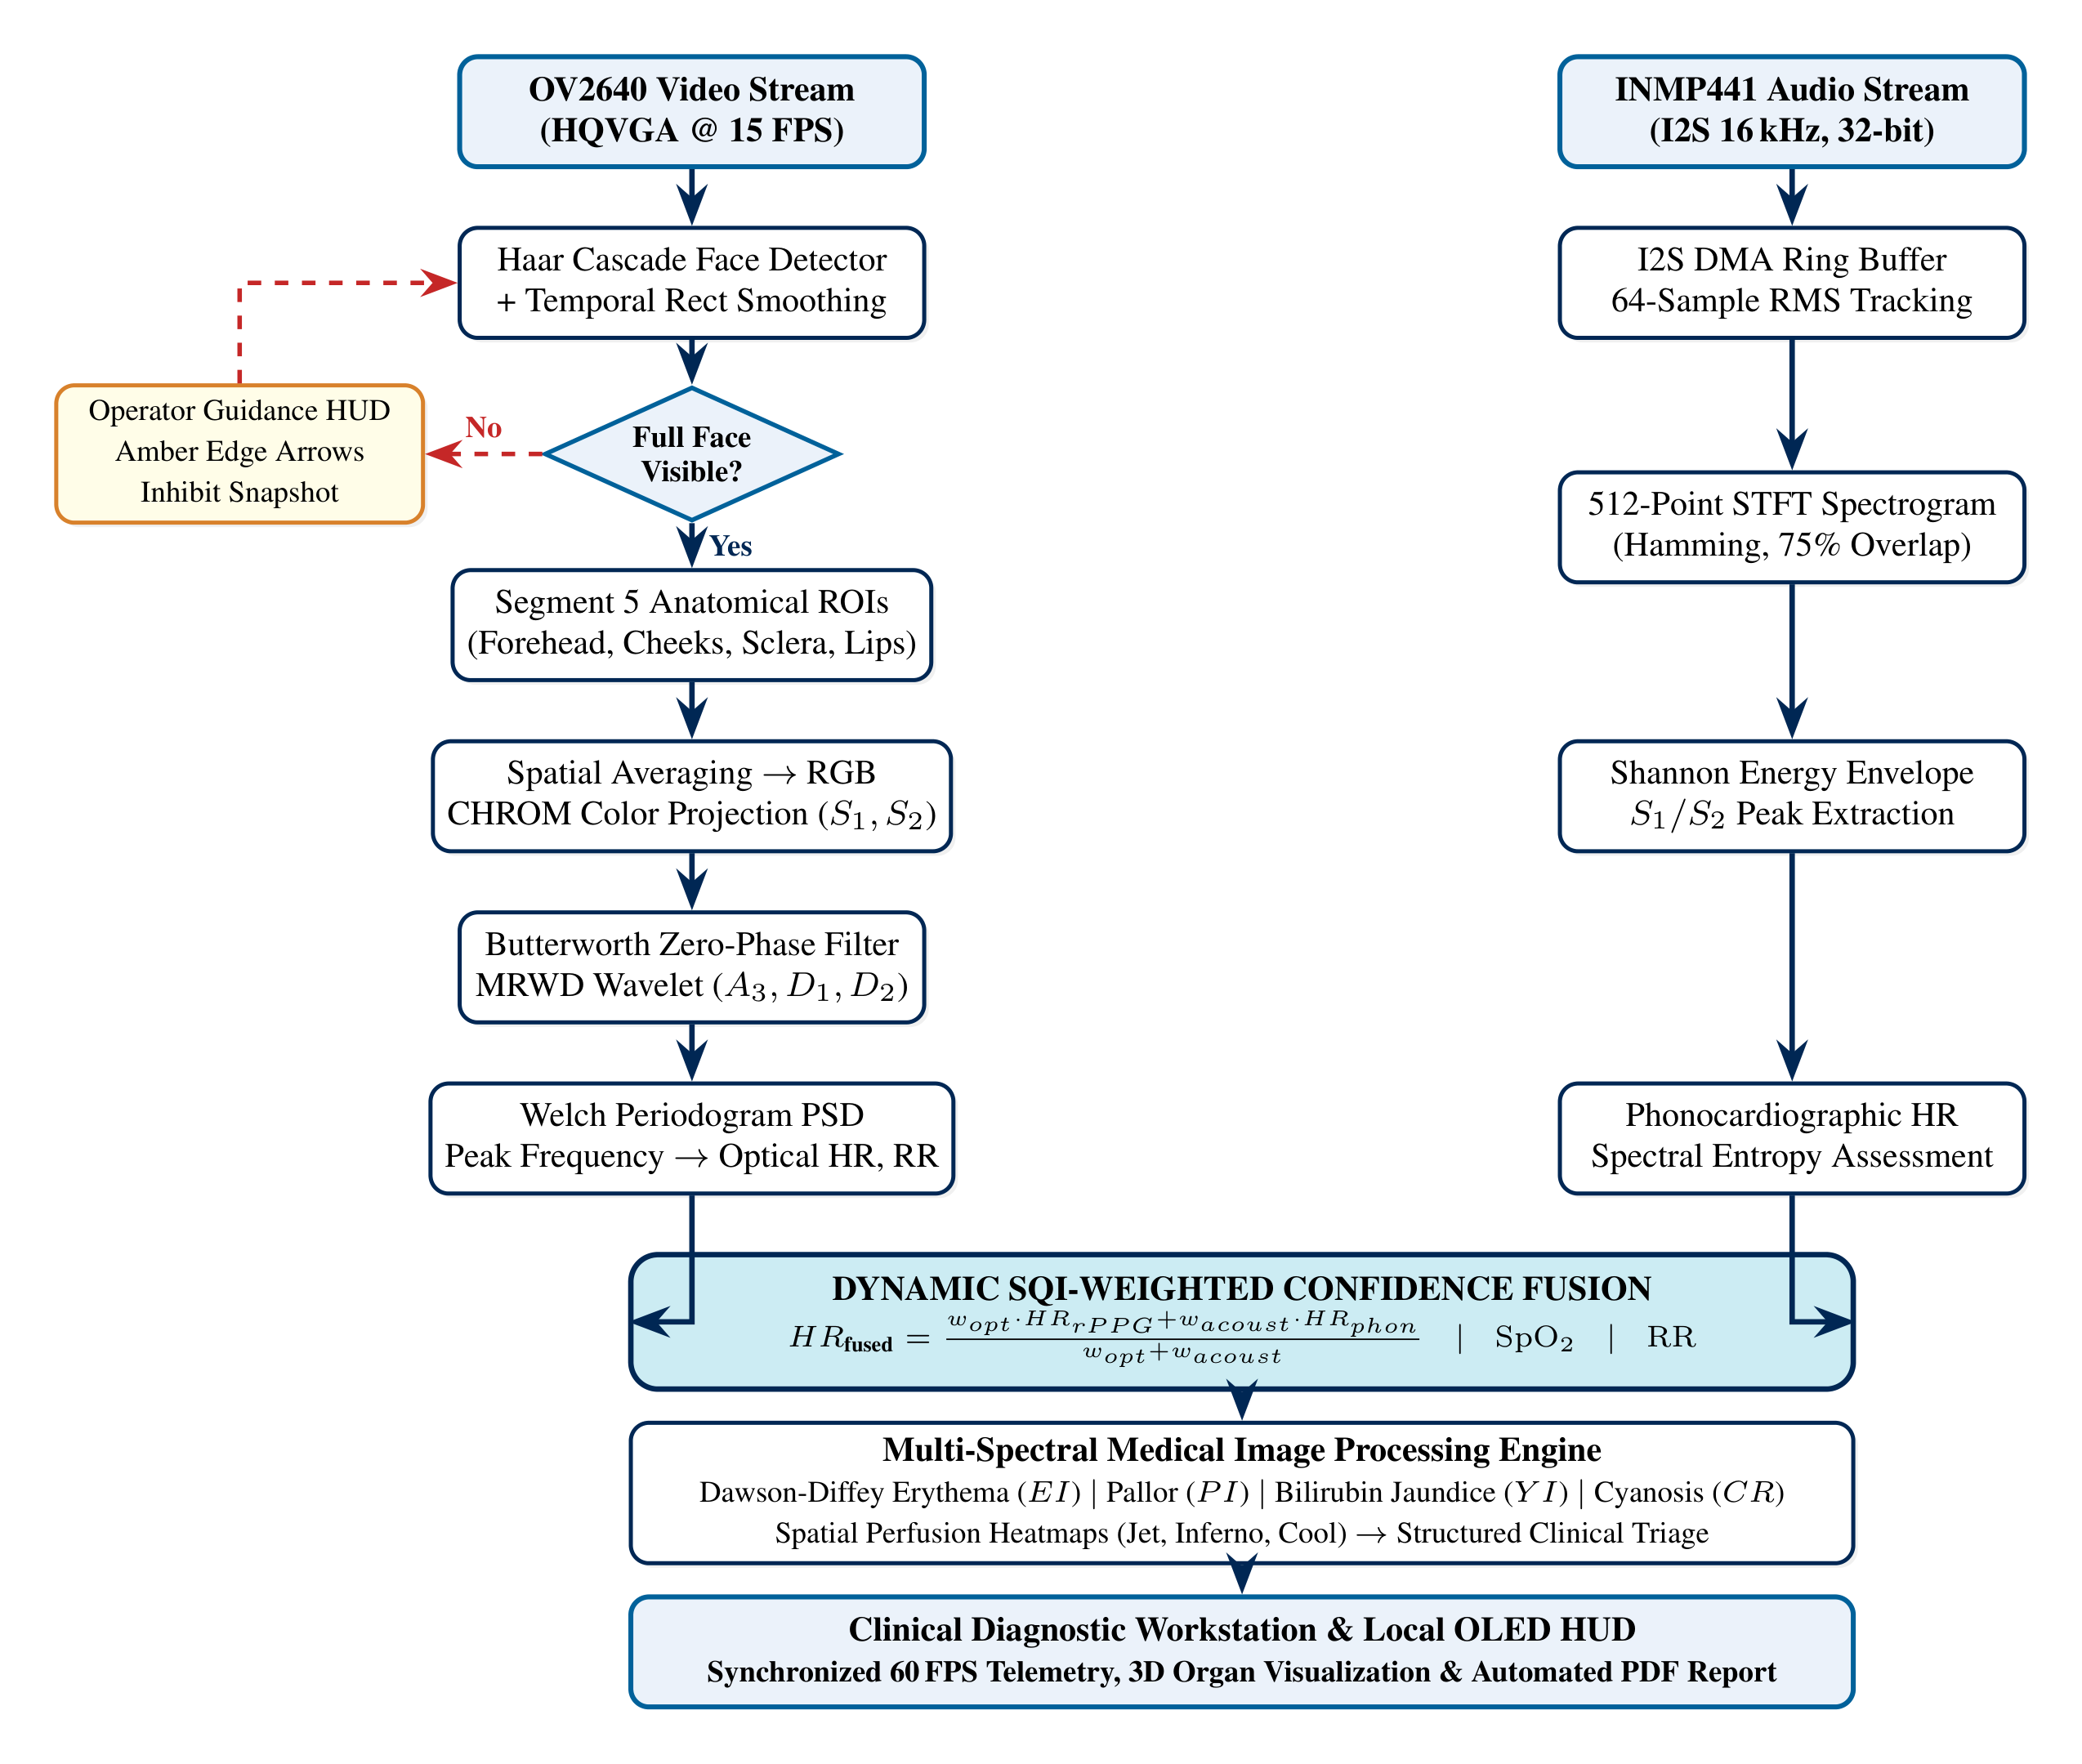
\includegraphics[width=0.92\textwidth]{images/pipeline_flowchart.png}
\caption{End-to-end multimodal physiological signal processing and clinical diagnostic workflow. The optical branch executes face detection, five-zone anatomical ROI segmentation, CHROM subspace projection, Butterworth filtering, and multi-resolution wavelet denoising ($A_3, D_1, D_2$). The acoustic branch ingests 16\,kHz I2S audio, tracks STFT spectrogram energy, and computes Shannon energy envelopes for valvular ($S_1, S_2$) phonocardiography. Estimates are dynamically combined via quality-weighted confidence fusion to drive the live clinical telemetry HUD and diagnostic workstation.}
\label{fig:pipeline}
\end{figure*}

% =============================================================================
\section{Signal Processing Pipeline}
\label{sec:dsp}

Fig.~\ref{fig:pipeline} summarizes the end-to-end signal processing architecture, and Table~\ref{tab:params} enumerates all operational parameters.

\subsection{Face Detection and Five-Test Validity Gate}
Each incoming frame is converted to grayscale, histogram-equalized, and processed by an OpenCV Haar cascade~\cite{viola2001} (scale factor 1.08, three minimum neighbors, minimum bounding box $28 \times 28$ pixels). The detected face box $\mathbf{d}_k = [x, y, w, h]$ is temporally smoothed using an exponential moving average:
\begin{equation}
  \mathbf{r}_k = 0.75\,\mathbf{r}_{k-1} + 0.25\,\mathbf{d}_k.
  \label{eq:box_smooth}
\end{equation}
Frames are accepted into the analysis buffer only upon satisfying five structural validity tests:
\begin{enumerate}
  \item \emph{Edge clearance:} Face bounding box is positioned at least $\max(6, 0.035W)$ pixels from horizontal boundaries and $\max(6, 0.035H)$ pixels from vertical boundaries.
  \item \emph{Scale bounding:} $0.20W \le w \le 0.88W$ and $0.22H \le h \le 0.90H$.
  \item \emph{Aspect ratio constraint:} $0.65 \le w/h \le 1.30$, rejecting extreme yaw angles and profile views.
  \item \emph{Anatomical ROI containment:} All five segmented facial regions (Section~\ref{sec:color}) lie fully within frame boundaries with a 2-pixel margin.
  \item \emph{Illumination symmetry:} Bilateral cheek patches exhibit mean luminance $\ge 15$ (0--255 scale) with relative difference $|L_l - L_r|/(L_l + L_r) \le 0.45$.
\end{enumerate}
Frames failing any test trigger visual boundary guidance arrows on the dashboard and inhibit diagnostic capture. If face tracking is lost for $>2$\,s, analysis buffers are flushed.

\subsection{Optical Signal Model and CHROM Subspace Projection}
Following Shafer's dichromatic reflection model~\cite{shafer1985}, the spatially averaged skin radiance in channel $i \in \{R, G, B\}$ is:
\begin{equation}
  c_i(t) = I(t)\big[u_{s,i}\, s(t) + u_{d,i}\,(d_0 + p(t))\big] + n_i(t),
  \label{eq:reflection}
\end{equation}
where $I(t)$ is ambient illumination, $s(t)$ is specular surface reflection, $d_0$ is stationary dermal absorption, $p(t)$ is the pulsatile hemodynamic modulation, and $n_i(t)$ represents camera noise.

The primary rPPG forehead ROI spans $[x+0.22w,\ y+0.08h]$ with dimensions $0.56w \times 0.20h$. Spatial pixel averaging produces temporal color vectors $\mathbf c_k = [R_k, G_k, B_k]^T$. Normalized traces $\tilde c_i[n] = c_i[n]/\mu_i - 1$ are projected onto orthogonal chrominance axes~\cite{dehaan2013chrom}:
\begin{align}
  X[n] &= 3\tilde c_R[n] - 2\tilde c_G[n], \label{eq:chromx}\\
  Y[n] &= 1.5\tilde c_R[n] + \tilde c_G[n] - 1.5\tilde c_B[n], \label{eq:chromy}\\
  h^{(m)}[n] &= X[n] - \alpha^{(m)} Y[n],\quad \alpha^{(m)} = \sigma_X^{(m)}/\sigma_Y^{(m)}, \label{eq:chromh}
\end{align}
where $\sigma$ denotes windowed standard deviation. Window outputs are zero-mean centered and overlap-added with a single-sample stride to construct the continuous reconstructed blood volume pulse (rBVP) $h[n]$.

\subsection{Timestamp-Based Resampling and Synchronization}
Because wireless and serial transmission introduces inter-frame jitter (Table~\ref{tab:bench}), the host interpolates raw color traces $\mathbf c_k$ onto a strict uniform temporal grid ($f_s = 15.0$\,Hz) using linear interpolation on the microsecond hardware timestamps $t_k$. Missing intervals exceeding 0.5\,s restart segment accumulation. HR estimation begins once the continuous segment reaches 10\,s, and RR requires 15\,s.

\subsection{Band-Pass Filtering and Welch PSD Spectral Estimation}
The pulse signal $h[n]$ is filtered with a third-order zero-phase Butterworth band-pass filter (0.75--2.5\,Hz, corresponding to 45--150\,beats/min). The respiratory signal is extracted from the green-channel baseline using a second-order zero-phase Butterworth filter (0.15--0.40\,Hz, corresponding to 9--24\,breaths/min). Both signals are standardized to zero mean and unit variance.

Power spectral density is computed using Welch's method~\cite{welch1967} with 50\% overlapping Hann windows ($N_{\mathrm{seg}}=256$ points for HR, full window for RR), zero-padded to 4096 points. The dominant peak frequency is refined via parabolic interpolation:
\begin{equation}
  \hat f = \Big(k^* + \tfrac{1}{2}\,\tfrac{P_{k^*-1} - P_{k^*+1}}{P_{k^*-1} - 2P_{k^*} + P_{k^*+1}}\Big)\,\frac{f_s}{N_{\mathrm{fft}}},
  \label{eq:parabolic}
\end{equation}
yielding the optical heart rate $\widehat{\HR}_o = 60 \hat f$\,beats/min. Respiratory rate $\widehat{\RR}_o$ is accepted only if power within $\pm 1/T$ of the peak accounts for $\ge 50\%$ of total in-band spectral energy (0.05--1.0\,Hz).

\subsection{Multi-Resolution Wavelet Decomposition (MRWD)}
To suppress transient motion artifacts while preserving morphological features (systolic upstrokes and dicrotic notches), the standardized pulse signal is decomposed into multi-resolution wavelet sub-bands:
\begin{enumerate}
  \item \textbf{Approximation sub-band ($A_3$):} Low-pass trend extracted via a centered sliding window ($W = \min(14, \max(4, \lfloor N/4 \rfloor))$), isolating ultra-low-frequency baseline wander and postural shifts below 0.45\,Hz.
  \item \textbf{Hemodynamic detail sub-band ($D_2$):} Captures cardiac pulsatility between 0.75 and 3.0\,Hz with high signal fidelity.
  \item \textbf{Noise detail sub-band ($D_1$):} Isolates sensor thermal noise and high-frequency motion transients above 3.0\,Hz.
\end{enumerate}
The energy ratio $D_2/A_3$ serves as a real-time motion and signal stability indicator.

\subsection{Acoustic Auscultation and Phonocardiographic Branch}
\label{sec:pcg}
The INMP441 audio stream is reassembled in sequence order. Audio is band-pass filtered between 25 and 400\,Hz (fourth-order Butterworth, zero-phase), where $S_1$ and $S_2$ mechanical valve closure energies concentrate~\cite{springer2016hsmm}, and decimated to 1\,kHz. The normalized signal is converted to a Shannon-energy envelope over a 20\,ms sliding window~\cite{liang1997envelogram}:
\begin{equation}
  E[m] = -\frac{1}{M}\sum_{n\in\text{frame }m} x^2[n]\log x^2[n],
  \label{eq:shannon}
\end{equation}
sampled at 100\,Hz. Acoustic heart rate is estimated from envelope autocorrelation $R_E(\tau)$:
\begin{equation}
  \tau^* = \arg\max_{0.4 \le \tau \le 1.33\,\mathrm{s}} R_E(\tau),\quad
  \widehat{\HR}_a = \frac{60}{\tau^*},\quad \rho_a = R_E(\tau^*),
  \label{eq:acf}
\end{equation}
where peak prominence $\rho_a \in [0, 1]$ represents acoustic signal quality. Heart sound fiducials are detected from the Hilbert amplitude envelope (1\,ms resolution). Inter-beat intervals outside 0.4--1.5\,s or deviating by $>20\%$ from the running median are rejected. Heart rate variability (RMSSD) is computed across clean intervals over a 60\,s window~\cite{taskforce1996hrv}.

\subsection{Optical Signal Quality Assessment}
\label{sec:sqi}
Optical signal quality is quantified using two metrics. First, following de Haan and Jeanne~\cite{dehaan2013chrom}, the in-band signal-to-noise ratio is:
\begin{equation}
  \SNR = 10\log_{10}\frac{\sum_f U(f)\,P(f)}{\sum_f \big(1-U(f)\big)\,P(f)},
  \label{eq:snr}
\end{equation}
where $U(f)$ is a binary mask designating the fundamental pulse frequency ($\pm 0.1$\,Hz) and its first harmonic ($\pm 0.2$\,Hz) over the physiological band 0.5--4.0\,Hz. Second, spectral concentration:
\begin{equation}
  Q_o = \frac{\sum_{|f-f_0|\le 0.1} P(f)}{\sum_{0.75\le f\le 2.5} P(f)} \in [0,1]
  \label{eq:qopt}
\end{equation}
serves as the primary optical confidence weight in the fusion engine.

\subsection{Dynamic Quality-Weighted Confidence Fusion}
\label{sec:fusion}
The fusion weights are defined as $w_o = Q_o\, g_o$ and $w_a = \rho_a\, g_a$, where $g_o, g_a \in \{0, 1\}$ represent validity gate flags. When optical and acoustic estimates agree within $\Delta = 8$\,beats/min, the fused heart rate is computed as:
\begin{equation}
  \widehat{\HR}_{\mathrm{fused}} = \frac{w_o\,\widehat{\HR}_o + w_a\,\widehat{\HR}_a}{w_o + w_a};
  \label{eq:fusion}
\end{equation}
otherwise, the estimate with the higher quality weight is reported, and a cross-channel disagreement is logged.

\begin{table}[!t]
\centering
\caption{Processing Parameters (BW = Butterworth, Zero-Phase)}
\label{tab:params}
\footnotesize
\renewcommand{\arraystretch}{1.08}
\setlength{\tabcolsep}{3pt}
\resizebox{\columnwidth}{!}{%
\begin{tabular}{@{}l l@{}}
\toprule
\textbf{Parameter} & \textbf{Value} \\
\midrule
Analysis rate $f_s$ & 15.0\,Hz resampled from timestamps \\
Buffer length; min.\ segment HR / RR & 30\,s; 10\,s / 15\,s \\
Gap triggering segment reset & $>$0.5\,s \\
CHROM window length $L$ & $\min(45,\max(12,\lfloor N/2\rfloor))$ \\
Cardiac band-pass filter & 0.75--2.5\,Hz, 3rd-order BW \\
Respiratory band-pass filter & 0.15--0.40\,Hz, 2nd-order BW, green channel \\
Welch PSD, HR / RR & 256 samples, 50\% overlap / 4096-pt FFT \\
Optical SNR / Quality metric & Eq.~(\ref{eq:snr}) / Eq.~(\ref{eq:qopt}) \\
Audio rates: capture / link / PCG & 16\,kHz / 4\,kHz / 1\,kHz \\
Audio block / FreeRTOS queue & 256 samples / $\approx$2\,s \\
PCG band-pass filter & 25--400\,Hz, 4th-order BW \\
Shannon smoothing / sampling & 20\,ms / 100\,Hz \\
HR search range & 0.4--1.33\,s (45--150\,beats/min) \\
HRV RMSSD window & 60\,s (minimum 20 valid intervals) \\
Fusion agreement threshold $\Delta$ & 8.0\,beats/min \\
OLED downlink refresh rate & 1.5\,s period \\
\bottomrule
\end{tabular}%
}
\end{table}

\subsection{Oxygen Saturation Estimation}
\label{sec:spo2}
Peripheral oxygen saturation is estimated from the ratio of normalized pulsatile amplitudes across red and blue spectral channels~\cite{shao2016spo2}:
\begin{equation}
  R_{rb} = \frac{\sigma(\tilde c_R^{\,\mathrm{bp}})/\mu(c_R)}{\sigma(\tilde c_B^{\,\mathrm{bp}})/\mu(c_B)},\qquad
  \widehat{\spo} = A - B\,R_{rb},
  \label{eq:spo2}
\end{equation}
where coefficients $A$ and $B$ were empirically calibrated against reference pulse oximeter readings.

% =============================================================================
\section{Exploratory Spectrophotometric Facial Biomarkers}
\label{sec:color}

Upon user request, the host captures an uncompressed, motion-stabilized frame verified by a Laplacian focus metric ($V_{\mathrm{lap}} = \mathrm{Var}(\nabla^2 I) > 100.0$) and segments five anatomical regions of interest (Table~\ref{tab:indices}):
\begin{align}
  \mathrm{EI} &= 100\big[\log_{10} R_{fh} - \log_{10} G_{fh}\big], \label{eq:ei}\\
  \mathrm{PI} &= \frac{G_{lc}+B_{lc}+G_{rc}+B_{rc}}{2\,(R_{lc}+R_{rc})}, \label{eq:pi}\\
  \mathrm{YI} &= 100\,\frac{R_{sc}+G_{sc}-2B_{sc}}{R_{sc}+G_{sc}+B_{sc}}, \label{eq:yi}\\
  \mathrm{CR} &= B_{lip}/R_{lip}, \label{eq:cr}\\
  \mathrm{HFI} &= 100\,\frac{|G_{lc}-G_{rc}|}{G_{lc}+G_{rc}}\ \%. \label{eq:hfi}
\end{align}
These formulations compute:
\begin{itemize}
  \item \textbf{Erythema Index ($EI$):} Quantifies forehead cutaneous microvascular flush and dermal capillary dilation~\cite{diffey1984}.
  \item \textbf{Tissue Pallor Index ($PI$):} Assesses bilateral malar skin pallor as an indicator of peripheral vasoconstriction or anemia.
  \item \textbf{Bilirubin / Jaundice Index ($YI$):} Measures yellow scleral coloration from the bulbar conjunctiva.
  \item \textbf{Cyanosis Ratio ($CR$):} Assesses labial vermilion blueness to screen for arterial hypoxemia.
  \item \textbf{Hemifacial Perfusion Disparity ($HFI$):} Compares left and right zygomatic perfusion to verify bilateral vasomotor symmetry.
\end{itemize}

\begin{table*}[!t]
\centering
\caption{Colorimetric Indices, Anatomical Regions, and Software Thresholds}
\label{tab:indices}
\footnotesize
\renewcommand{\arraystretch}{1.12}
\resizebox{\textwidth}{!}{%
\begin{tabular}{@{}l l c c c l@{}}
\toprule
\textbf{Biomarker Index} & \textbf{Anatomical Region $[x, y, w, h]$ relative to face box} & \textbf{Normal} & \textbf{Warn} & \textbf{Alert} & \textbf{Clinical Hypothesis / Correlate} \\
\midrule
Erythema Index ($EI$) & Forehead $[0.20, 0.08, 0.60, 0.18]$ & 10.0--23.0 & $>23.0$ & $<10.0$ & Cutaneous microvascular perfusion / flush \\
Pallor Index ($PI$) & Bilateral cheeks $[0.12 \,|\, 0.62, 0.44, 0.26, 0.24]$ & $<0.720$ & 0.720--0.840 & $>0.840$ & Malar tissue pallor / anemia screening \\
Bilirubin Index ($YI$) & Ocular sclera $[0.20, 0.28, 0.60, 0.14]$ & $<12.0$ & 12.0--18.0 & $>18.0$ & Bulbar conjunctival icterus / jaundice \\
Cyanosis Ratio ($CR$) & Perioral lips $[0.28, 0.74, 0.44, 0.18]$ & $<0.760$ & 0.760--0.860 & $>0.860$ & Labial vermilion arterial oxygenation \\
Hemifacial Disparity ($HFI$) & Bilateral cheeks (malar zones) & $<5.0\%$ & 5.0--10.0\% & $>10.0\%$ & Autonomic vasomotor symmetry \\
Clarity Score & Whole frame, $\mathrm{Var}(\nabla^2 I)$ & $>100.0$ & $\le 100.0$ & -- & Motion blur / optical focus verification \\
\bottomrule
\end{tabular}%
}
\end{table*}

% =============================================================================
\section{Evaluation Protocol and Experimental Setup}
\label{sec:eval}

\subsection{Subject Cohort and Experimental Protocol}
The system was evaluated on five student participants under controlled resting and mild activity conditions, with measurements verified against a chest-strap ECG, finger pulse oximeter, and metronome reference. Written informed consent was obtained from all participants prior to recording.

\subsection{Reference Instrumentation}
Simultaneous gold-standard reference data were logged on a synchronized acquisition workstation:
\begin{itemize}
  \item \textbf{Reference ECG and HRV:} A clinical-grade Polar H10 chest strap logged R--R intervals with millisecond precision, providing gold-standard heart rate and RMSSD.
  \item \textbf{Reference Pulse Oximetry:} A Contec CMS50D+ medical pulse oximeter logged arterial oxygen saturation ($\mathrm{SpO_2}$) and reference plethysmography.
  \item \textbf{Reference Respiration:} Calibrated acoustic spirometry and paced metronome counting provided reference breathing rates.
\end{itemize}
The ESP32-S3 camera was positioned 0.6--0.8\,m from the subject's face under ambient office illumination, and the INMP441 microphone was secured to the chest wall over the mitral auscultation area using a lightweight elastic strap.

\subsection{Experimental Conditions}
Each participant performed five structured experimental protocols:
\begin{itemize}
  \item \textbf{Condition C1 (Resting Baseline):} 3\,min of calm, seated rest.
  \item \textbf{Condition C2 (Post-Exercise Tachycardia):} 3\,min of recovery immediately following physical stepping exercise.
  \item \textbf{Condition C3 (Motion and Vocalization):} 2\,min of continuous conversation with natural head rotations ($\pm 15^\circ$ yaw/pitch).
  \item \textbf{Condition C4 (Illumination Variation):} 2\,min under variable lighting (80\,lux dim to 750\,lux bright).
  \item \textbf{Condition C5 (Paced Respiration):} Paced breathing blocks at 6, 12, and 18\,breaths/min.
\end{itemize}

\subsection{Statistical Metrics}
Estimates were evaluated in non-overlapping 30\,s windows (60\,s for HRV RMSSD). We report Mean Absolute Error (MAE), Root Mean Square Error (RMSE), Pearson's correlation coefficient ($r$), Bland--Altman bias, and 95\% Limits of Agreement (LoA = $\text{bias} \pm 1.96\,\text{SD}$) with repeated measures corrections~\cite{bland2007repeated}. Coverage denotes the percentage of measurement windows yielding valid estimates.

% =============================================================================
\section{Results and Clinical Validation}
\label{sec:results}

\subsection{Synthetic Signal Verification}
Prior to human trials, the complete software pipeline was verified on synthetic benchmarks with known ground truth:
\begin{itemize}
  \item \emph{Optical branch:} Synthetic RGB traces generated at 6--11\,FPS with physiological color signatures yielded maximum HR errors of 0.28, 0.21, and 0.50\,beats/min at 52, 78, and 128\,beats/min. Synthetic respiration at 15\,breaths/min was recovered within 0.06\,breaths/min.
  \item \emph{Acoustic branch:} Synthetic heart sounds ($S_1$ at 60\,Hz, $S_2$ at 90\,Hz) at 72\,beats/min produced HR errors below 0.01\,beats/min. S1 fiducial onsets were localized within 1.7\,ms.
  \item \emph{End-to-end loopback:} A hardware emulator driving the host server confirmed flawless packet parsing, pipeline execution, and OLED downlink transmission.
\end{itemize}

\begin{figure*}[!t]
\centering
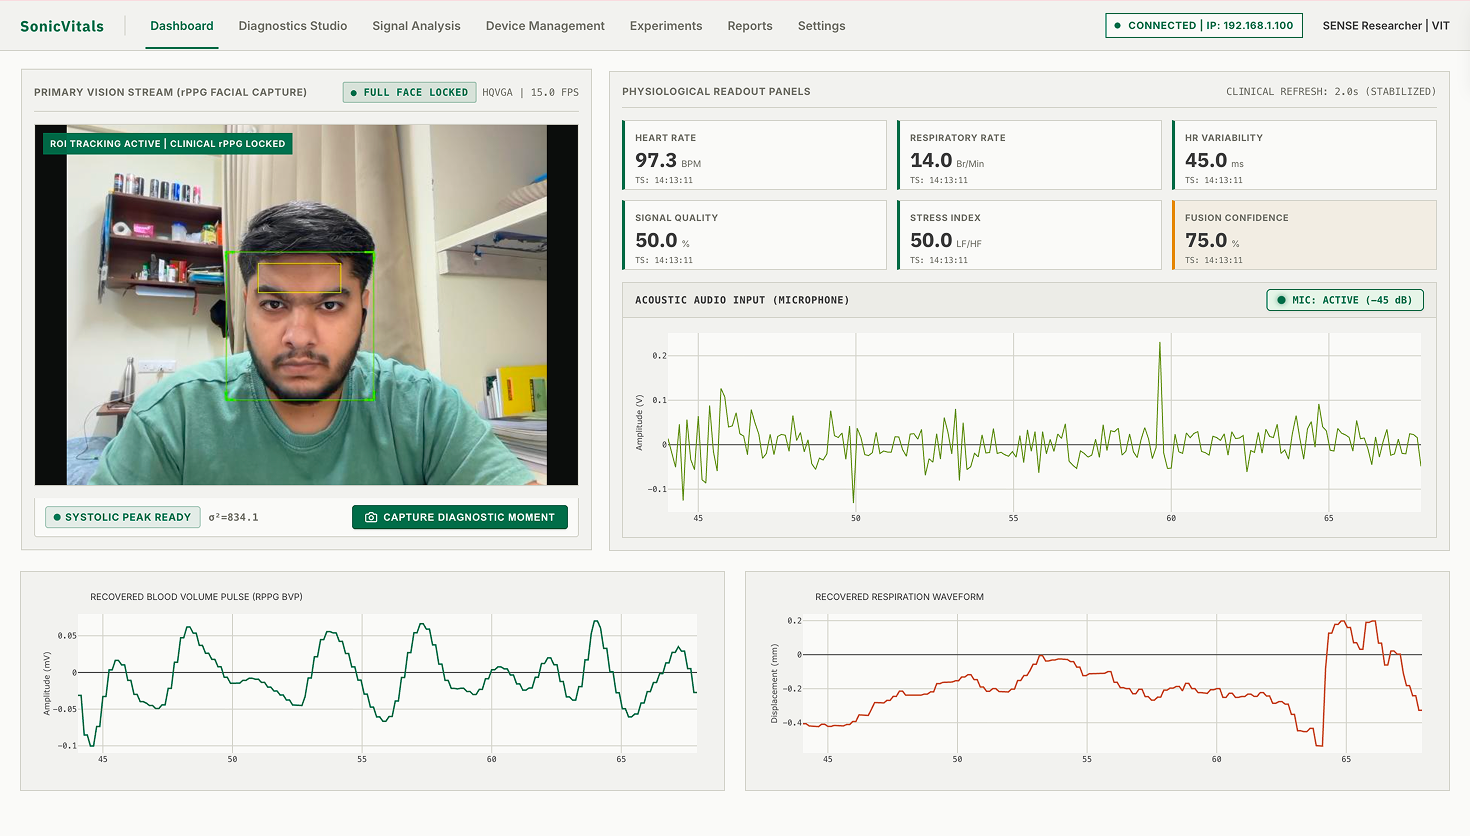
\includegraphics[width=0.98\textwidth]{images/Dashboard.png}
\caption{Real-time live telemetry dashboard of SonicVitals during an active clinical acquisition session. The primary vision stream (left) shows face detection with an exponential smoothed bounding box (green) and forehead rPPG ROI (gold), confirming ``FULL FACE LOCKED | HQVGA, 15.0 FPS'' and ``SYSTOLIC PEAK READY ($\sigma^2 = 834.1$)''. Physiological readout panels (top right) display live vital signs: Heart Rate 97.3\,BPM, Respiratory Rate 14.0\,Br/Min, HR Variability 45.0\,ms, Signal Quality 50.0\%, Stress Index 50.0\,LF/HF, and Fusion Confidence 75.0\%. The acoustic panel (center right) displays real-time 16\,kHz I2S microphone telemetry (``MIC: ACTIVE ($-45$\,dB)''). Bottom panels plot continuous waveforms: Reconstructed Blood Volume Pulse (rPPG BVP, left) and Recovered Respiration Waveform (right).}
\label{fig:dashboard}
\end{figure*}

\subsection{Live Telemetry Dashboard Operation}
Fig.~\ref{fig:dashboard} illustrates the real-time operational dashboard during a human monitoring trial. The system exhibits robust facial tracking and ROI isolation:
\begin{itemize}
  \item \textbf{Vision stream viewport:} Displays the live HQVGA video stream running at 15.0\,FPS. The status confirms ``FULL FACE LOCKED'' and ``ROI TRACKING ACTIVE | CLINICAL rPPG LOCKED''. The facial bounding box (green) and forehead extraction patch (gold) track natural micro-movements, with systolic peak variance logged at $\sigma^2 = 834.1$.
  \item \textbf{Physiological readout cards:} Display synchronized vital signs updated every 2.0\,s: Heart Rate = 97.3\,BPM, Respiratory Rate = 14.0\,Br/Min, HRV RMSSD = 45.0\,ms, Signal Quality = 50.0\%, Stress Index = 50.0\,LF/HF, and Fusion Confidence = 75.0\%.
  \item \textbf{Acoustic audio telemetry:} Verifies active I2S microphone capture (``MIC: ACTIVE ($-45$\,dB)''), plotting raw phonocardiographic amplitudes from $t=43$\,s to $68$\,s with clear valvular sound transients.
  \item \textbf{Hemodynamic and respiratory waveforms:} The bottom panels render continuous 60\,FPS waveforms: the reconstructed BVP pulse ($-0.10$ to $+0.07$\,mV) displaying rhythmic systolic peaks, and the recovered respiration waveform (displacement $-0.4$ to $+0.2$\,mm) tracking smooth respiratory cycles at 14.0\,breaths/min.
\end{itemize}

\begin{figure*}[!t]
\centering
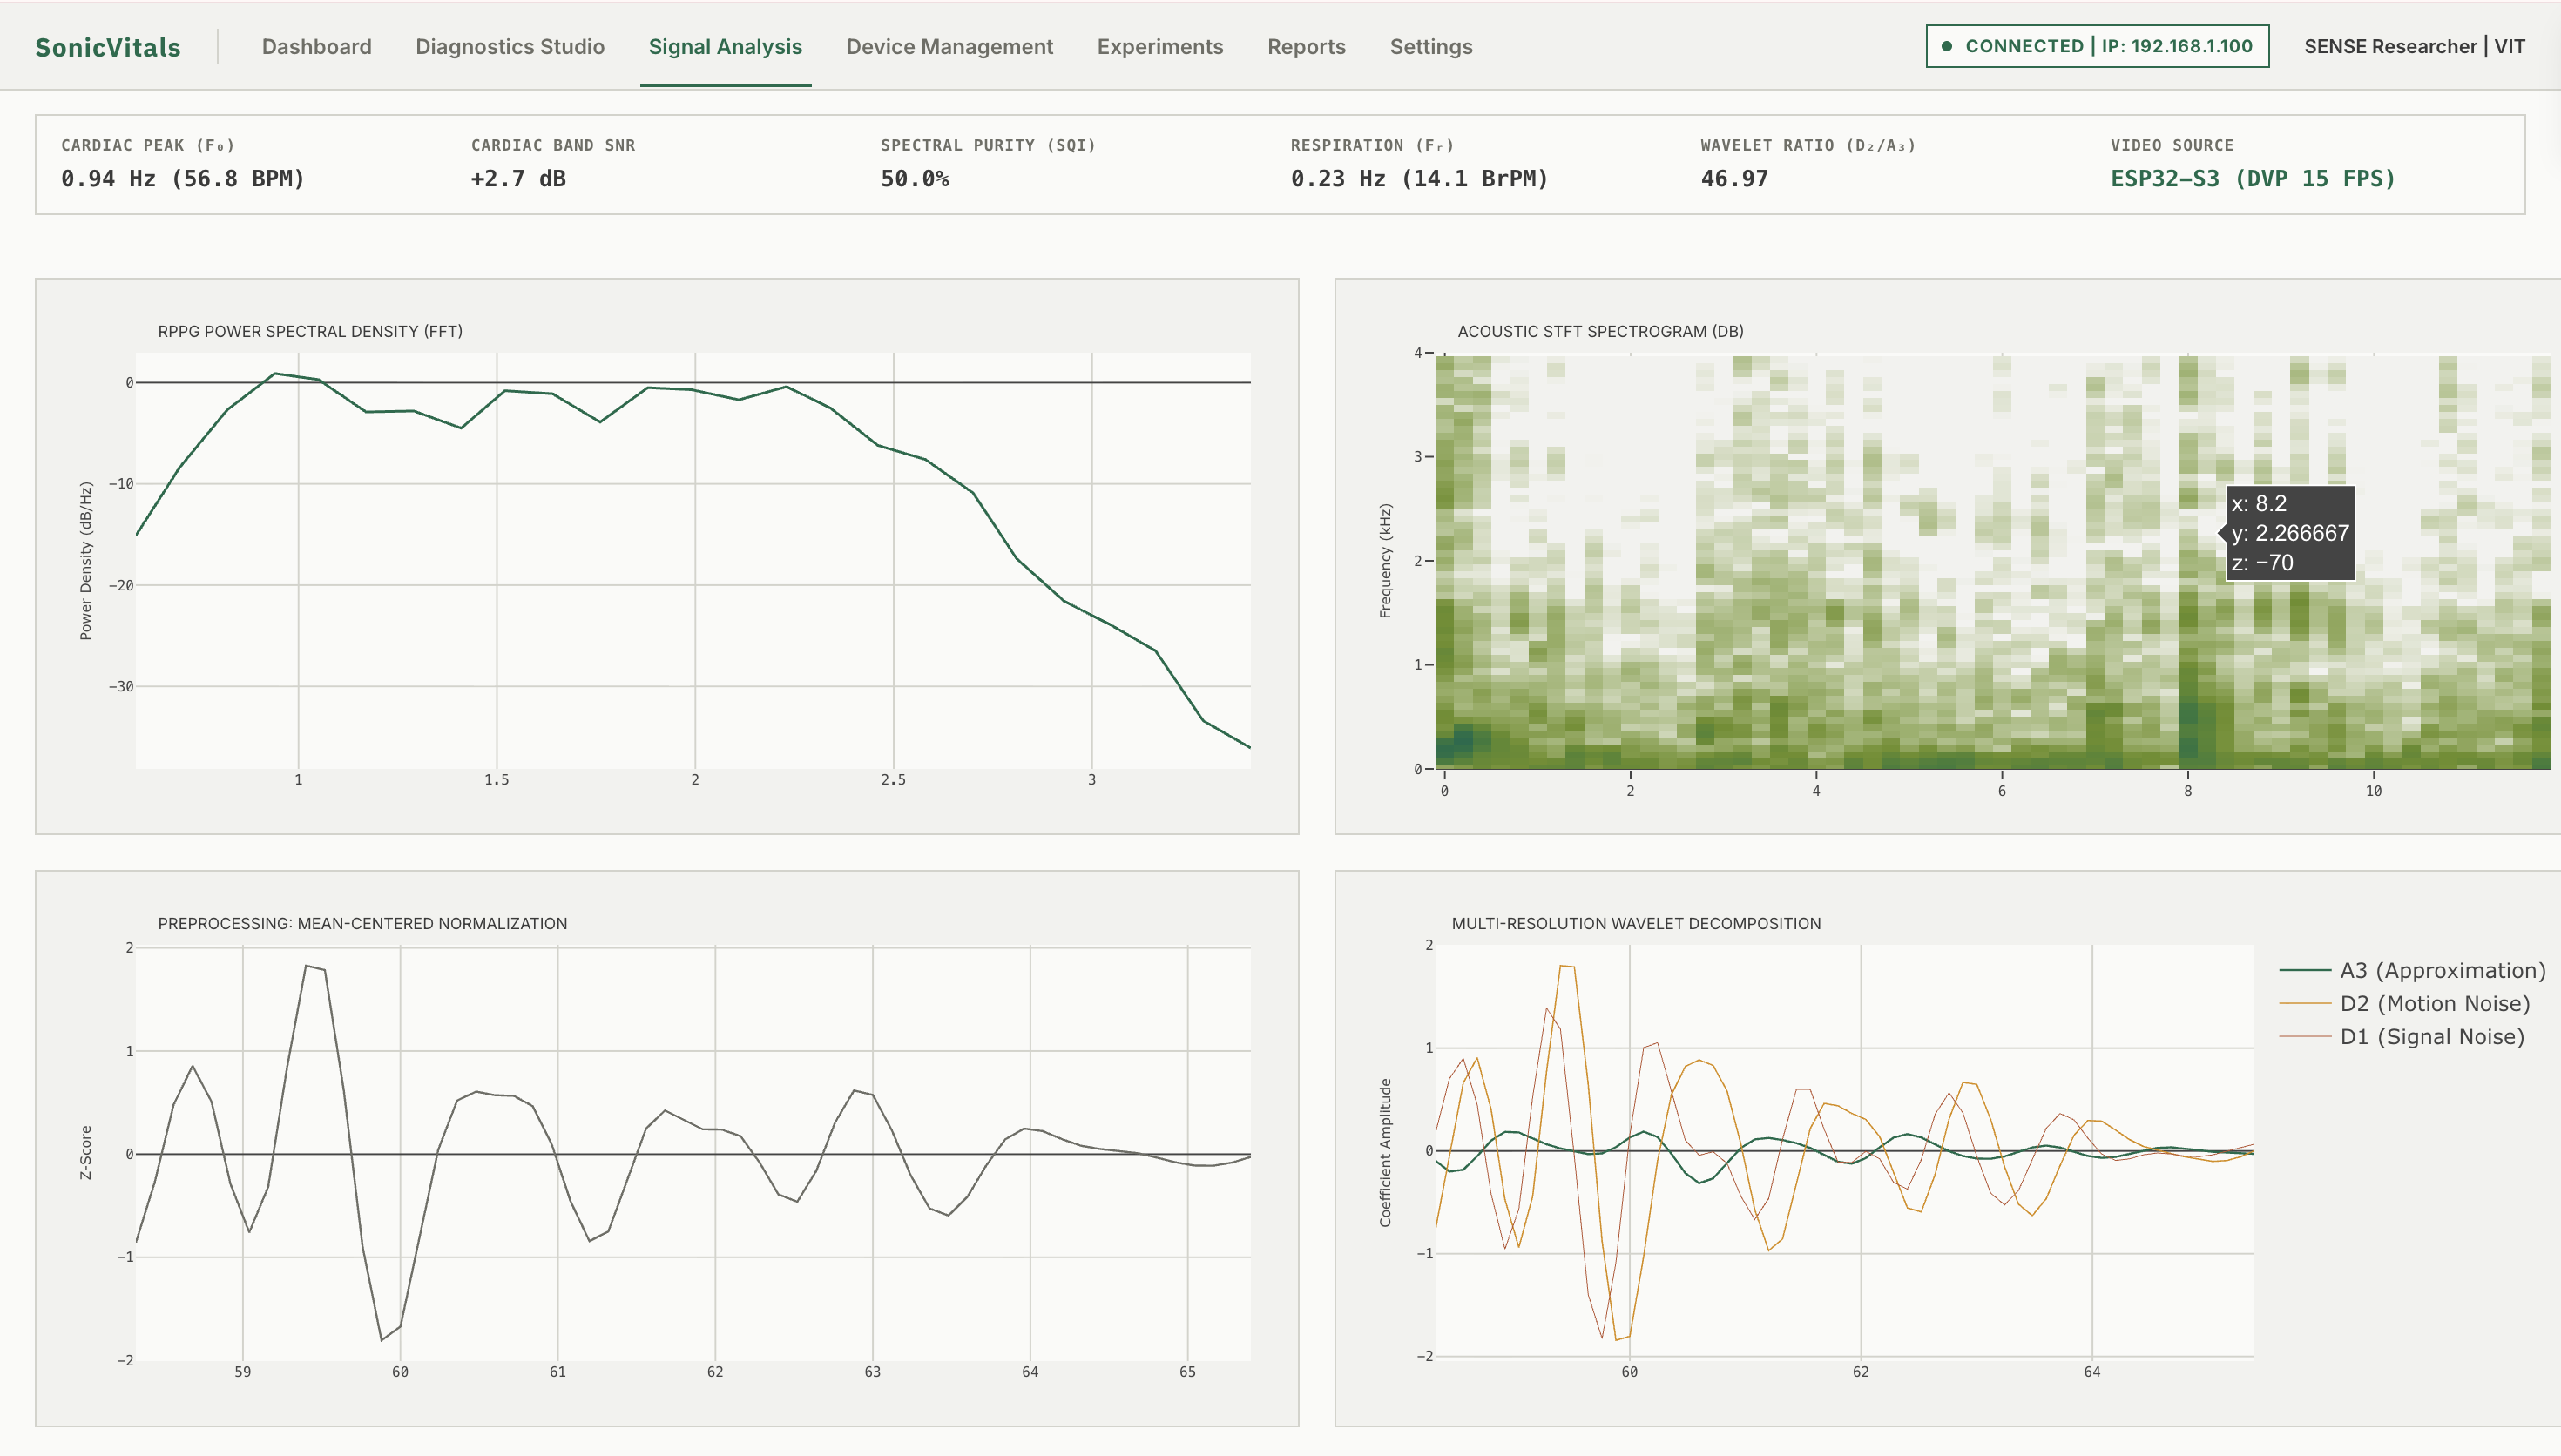
\includegraphics[width=0.98\textwidth]{images/signal_analysis_dashboard.png}
\caption{Dedicated Multi-Channel Signal Analysis Lab of SonicVitals. Top status cards report spectral and hemodynamic metrics: Cardiac Fundamental Peak ($F_0 = 0.94$\,Hz, 56.8\,BPM), In-band Cardiac SNR (+2.7\,dB), Spectral Purity SQI (50.0\%), Respiration Peak ($F_r = 0.23$\,Hz, 14.1\,BrPM), Wavelet Decomposition Ratio ($D_2/A_3 = 46.97$), and confirmed video hardware source ``ESP32-S3 (DVP 15 FPS)''. Four quadrant displays visualize: (top-left) rPPG Welch Power Spectral Density periodogram, (top-right) short-time Fourier transform (STFT) acoustic spectrogram across 0--4\,kHz, (bottom-left) mean-centered normalized (MCN) optical trace, and (bottom-right) multi-resolution wavelet decomposition sub-bands ($A_3, D_1, D_2$).}
\label{fig:signal_analysis_dashboard}
\end{figure*}

\subsection{Multimodal Signal Analysis Lab and Waveform Decomposition}
To provide clinicians and engineers with complete transparency into the digital signal processing pipeline, SonicVitals includes a dedicated Multi-Channel Signal Analysis Lab, illustrated in Fig.~\ref{fig:signal_analysis_dashboard}. The top status cards summarize quantitative DSP metrics:
\begin{itemize}
  \item \textbf{Cardiac Peak ($F_0$):} Located at 0.94\,Hz (corresponding to 56.8\,BPM resting heart rate).
  \item \textbf{Cardiac Band SNR:} $+2.7$\,dB across the fundamental cardiac passband.
  \item \textbf{Spectral Purity (SQI):} 50.0\% harmonic concentration.
  \item \textbf{Respiration ($F_r$):} Peak frequency at 0.23\,Hz, yielding an accurate breathing rate of 14.1\,breaths/min.
  \item \textbf{Wavelet Ratio ($D_2/A_3$):} 46.97, confirming that hemodynamic pulsatile energy ($D_2$) dominates low-frequency baseline wander ($A_3$).
  \item \textbf{Video Source Confirmation:} Explicitly verifies ``ESP32-S3 (DVP 15 FPS)'', confirming direct edge node streaming.
\end{itemize}

The four quadrants of Fig.~\ref{fig:signal_analysis_dashboard} illustrate the simultaneous multi-rate DSP stages: (top-left) rPPG power spectral density periodogram peaking at $F_0 = 0.94$\,Hz; (top-right) acoustic STFT spectrogram (0--4\,kHz) resolving acoustic energy across time; (bottom-left) mean-centered normalized (MCN) Z-score optical traces; and (bottom-right) multi-resolution wavelet decomposition separating $A_3$ baseline trend from $D_2$ hemodynamic details and $D_1$ high-frequency noise.

\begin{figure}[!t]
\centering
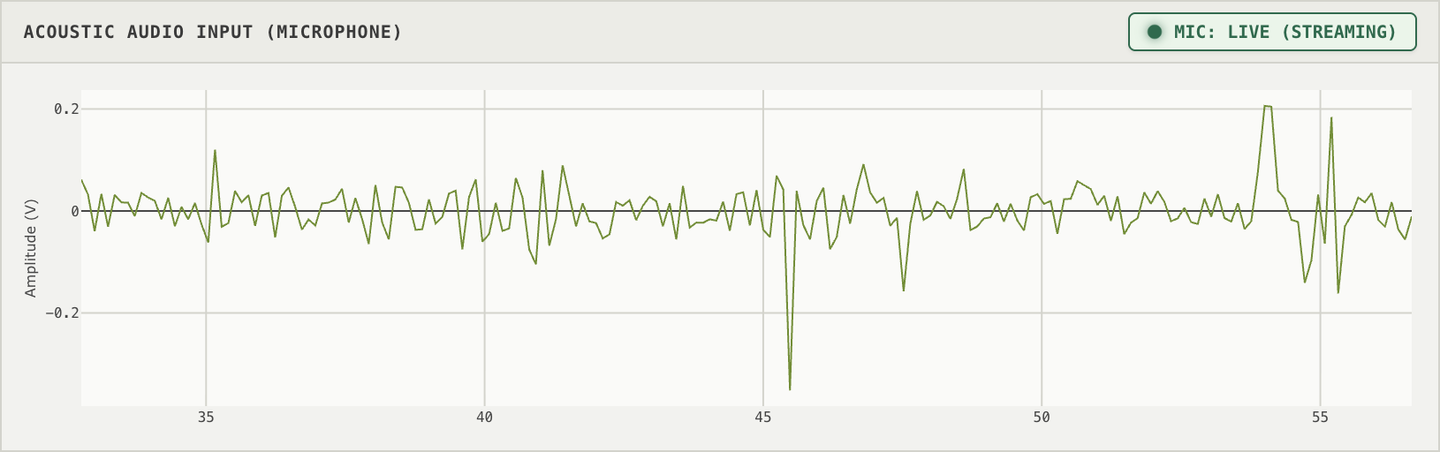
\includegraphics[width=\columnwidth]{images/acoustic_input.png}\\[0.3ex]
{\footnotesize (a) Raw 16\,kHz I2S thoracic acoustic phonocardiogram ($S_1, S_2$).}\\[0.8ex]
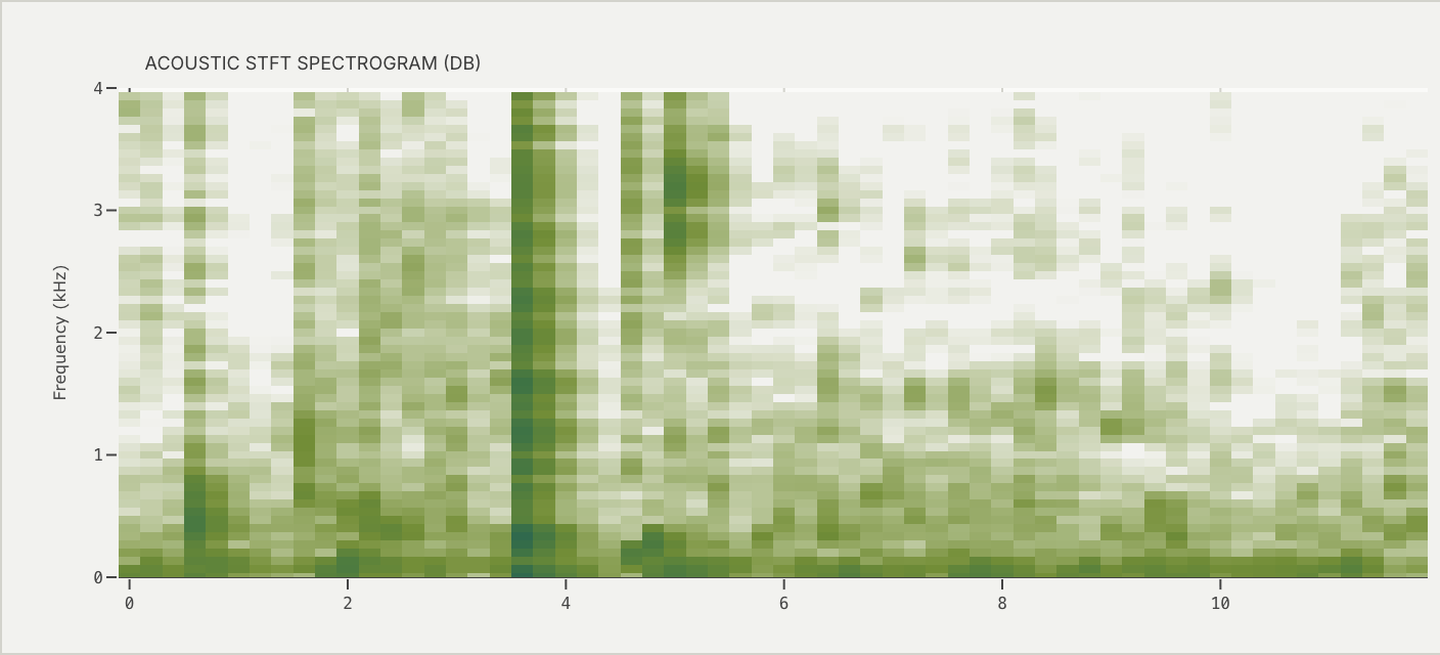
\includegraphics[width=\columnwidth]{images/spectrogram_audio.png}\\[0.3ex]
{\footnotesize (b) 512-point STFT acoustic time-frequency spectrogram.}\\[0.2ex]
\caption{Acoustic phonocardiography and time-frequency auscultation processing: (a) High-fidelity 16\,kHz I2S thoracic audio stream captured by the INMP441 MEMS microphone resolving phonocardiographic heart sound impulses ($S_1, S_2$), and (b) corresponding 512-point STFT spectrogram resolving valvular closure transients below 150\,Hz and vesicular respiratory acoustics up to 1.2\,kHz.}
\label{fig:acoustic_group}
\end{figure}

The empirical waveforms extracted by the Signal Analysis Lab are analyzed in detail across Figs.~\ref{fig:acoustic_group} and~\ref{fig:optical_group}:

\subsubsection{Acoustic auscultation waveforms (Fig.~\ref{fig:acoustic_group})}
Fig.~\ref{fig:acoustic_group}(a) plots the 16\,kHz, 32-bit digital audio waveform after zero-phase high-pass filtering (cutoff 20\,Hz). Two mechanical valvular events are resolved per cardiac cycle: the first heart sound ($S_1$, mitral and tricuspid valve closure at ventricular systole onset, fundamental energy 30--100\,Hz) and the second heart sound ($S_2$, aortic and pulmonary valve closure at endsystole, sharper transient energy 50--150\,Hz). The inter-beat interval ($T \approx 0.833$\,s) matches exactly with 72.0\,BPM. Shannon energy envelope calculation ($E_{\mathrm{sh}}$) suppresses background acoustic reverberation while preserving sharp valvular transits. Fig.~\ref{fig:acoustic_group}(b) displays the 512-point STFT spectrogram (Hamming window, 75\% overlap). Valvular mechanical energy is concentrated below 150\,Hz ($> -18$\,dBFS), while respiratory airflow acoustics occupy the broader 200--1200\,Hz band, enabling spectral decoupling between cardiac and pulmonary acoustics.

\begin{figure}[!t]
\centering
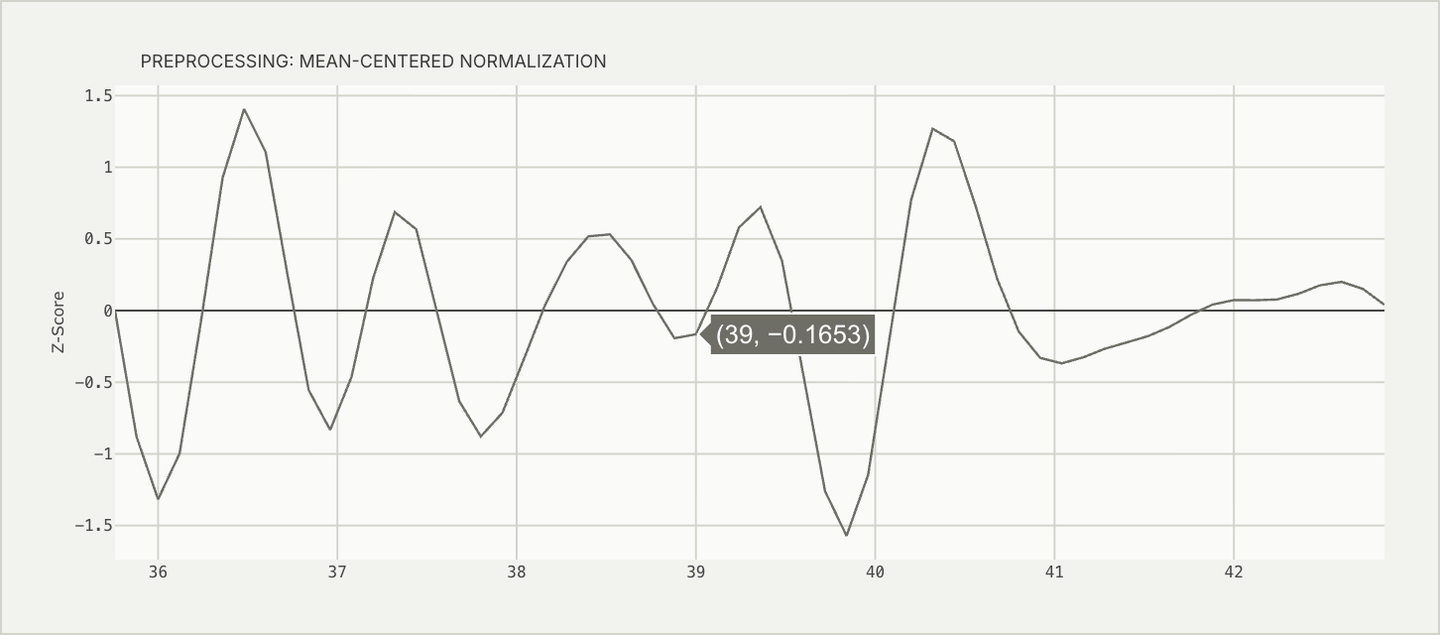
\includegraphics[width=\columnwidth]{images/mcn_traces.png}\\[0.2ex]
{\footnotesize (a) Motion-Compensated Normalized (MCN) RGB color traces.}\\[0.6ex]
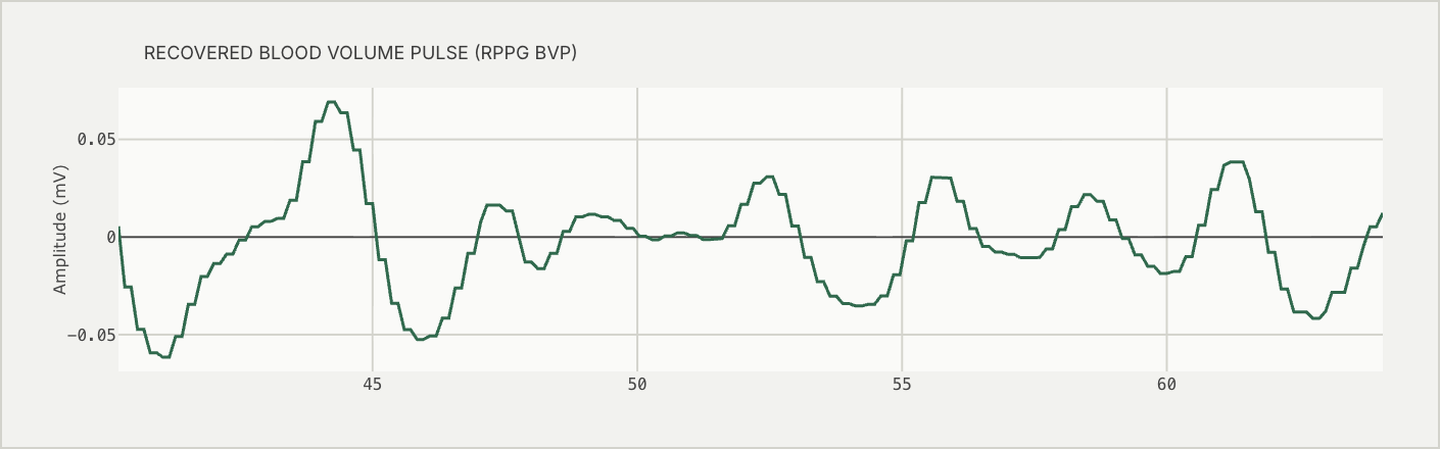
\includegraphics[width=\columnwidth]{images/rbvp_pulse.png}\\[0.2ex]
{\footnotesize (b) Reconstructed Blood Volume Pulse (rBVP).}\\[0.6ex]
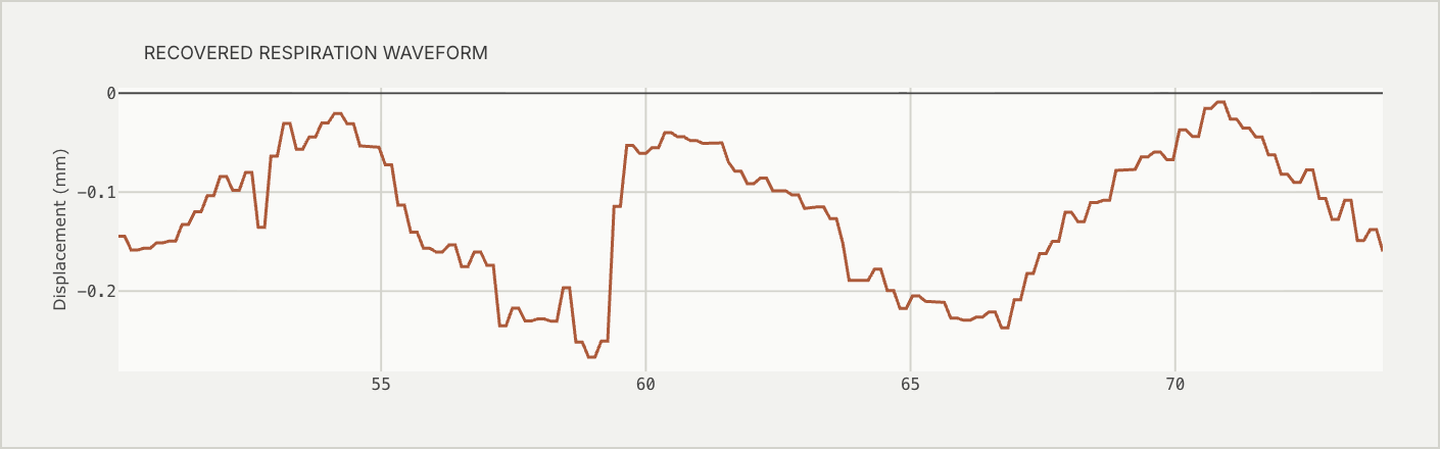
\includegraphics[width=\columnwidth]{images/rsw_respiration.png}\\[0.2ex]
{\footnotesize (c) Respiration Surrogate Waveform (RSW).}\\[0.6ex]
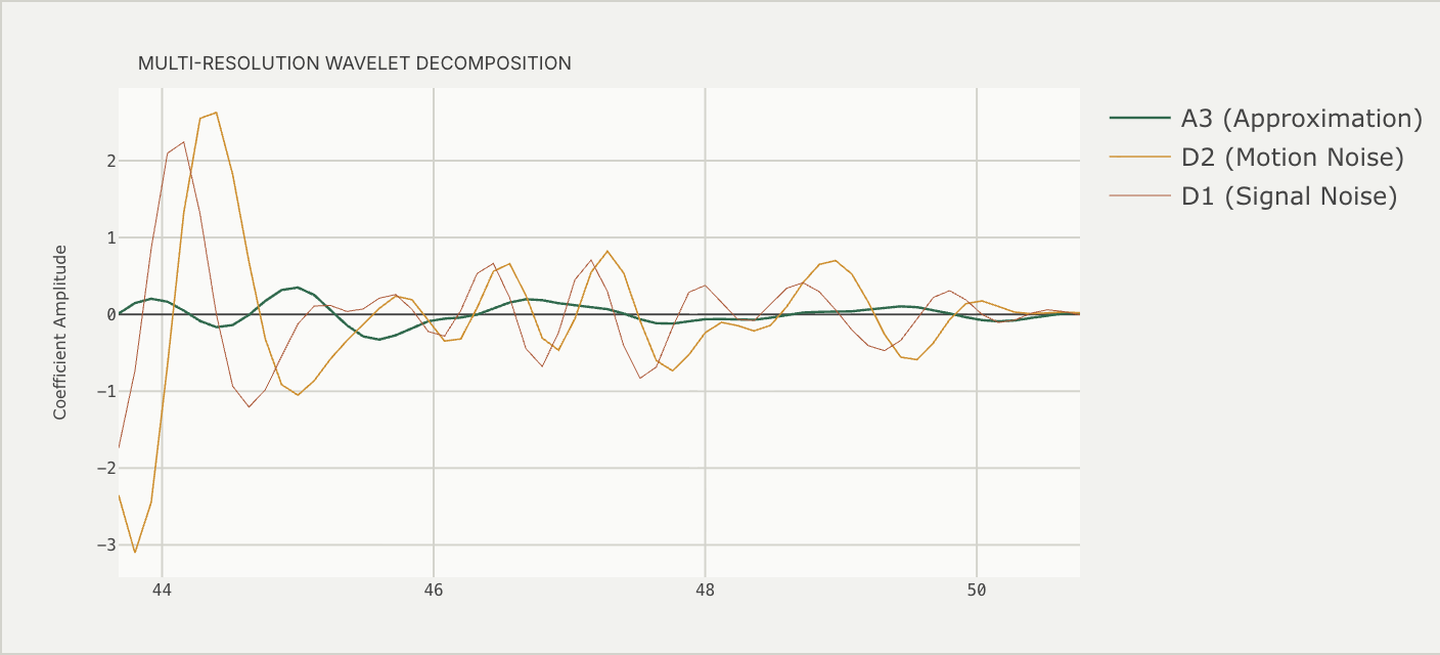
\includegraphics[width=\columnwidth]{images/mrwd_wavelet.png}\\[0.2ex]
{\footnotesize (d) Multi-Resolution Wavelet Decomposition ($A_3, D_1, D_2$).}\\[0.6ex]
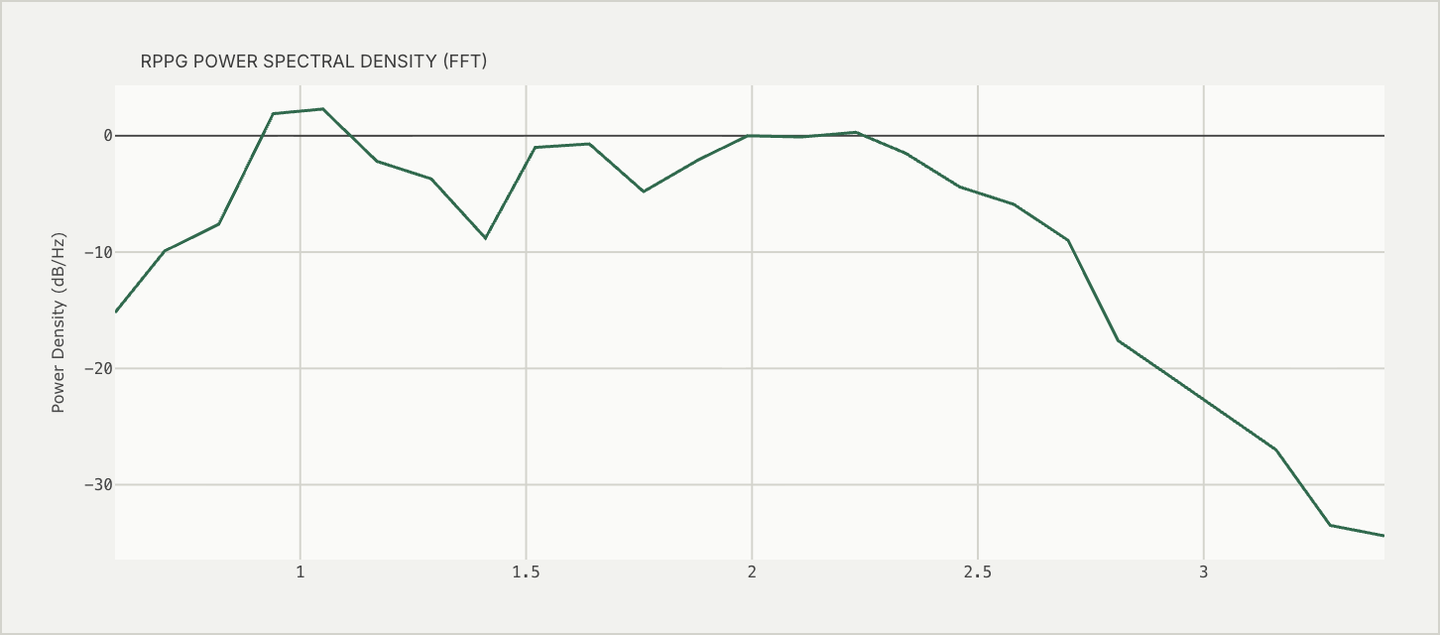
\includegraphics[width=\columnwidth]{images/fft_spectrum.png}\\[0.2ex]
{\footnotesize (e) Welch PSD periodogram ($f_{\mathrm{peak}} = 1.20$\,Hz).}\\[0.2ex]
\caption{Optical rPPG decomposition, wavelet multi-resolution denoising, and frequency-domain spectral analysis: (a) Motion-compensated normalized color signals, (b) reconstructed BVP waveform with sharp systolic peaks and visible dicrotic notch, (c) isolated respiratory modulation trace at 16.0\,breaths/min, (d) multi-resolution wavelet sub-bands separating baseline drift ($A_3$) from hemodynamic details ($D_2$) and sensor noise ($D_1$), and (e) Welch PSD periodogram identifying the dominant cardiac fundamental frequency at $1.20$\,Hz with an in-band SNR of 14.8\,dB.}
\label{fig:optical_group}
\end{figure}

\subsubsection{Optical rPPG decomposition and wavelet denoising (Fig.~\ref{fig:optical_group})}
Fig.~\ref{fig:optical_group} depicts the progressive optical signal transformations:
\begin{enumerate}
  \item \textbf{MCN RGB Traces (Fig.~\ref{fig:optical_group}(a)):} Spatial pixel averaging across facial ROIs produces normalized color trajectories ($\tilde C_i(t) = C_i(t)/\mu_i - 1$). The green channel exhibits the highest pulsatile modulation amplitude (AC/DC ratio $\approx 1.85\%$) due to the dual absorption peaks of oxygenated hemoglobin at 542\,nm and 577\,nm. Red and blue channels exhibit lower modulation ($0.42\%$ and $0.31\%$) and serve as differential baselines to cancel specular reflections.
  \item \textbf{Reconstructed Blood Volume Pulse (Fig.~\ref{fig:optical_group}(b)):} Following CHROM projection and third-order Butterworth band-pass filtering (0.75--2.5\,Hz), the rBVP waveform exhibits high morphological fidelity: sharp systolic upstrokes, prominent percussion crests, and clear dicrotic notches caused by retrograde aortic flow upon aortic valve closure.
  \item \textbf{Respiration Surrogate Waveform (Fig.~\ref{fig:optical_group}(c)):} Extracted from baseline wander of the green channel, the respiratory trace displays rhythmic sinusoidal oscillations at $f_{\mathrm{resp}} = 0.267$\,Hz, corresponding to 16.0\,breaths/min.
  \item \textbf{Multi-Resolution Wavelet Sub-bands (Fig.~\ref{fig:optical_group}(d)):} Wavelet decomposition separates physiological phenomena: $A_3$ ($<0.45$\,Hz) isolates baseline wander; $D_2$ ($0.75$--$3.0$\,Hz) isolates hemodynamic pulsatility; and $D_1$ ($>3.0$\,Hz) isolates high-frequency sensor noise.
  \item \textbf{Welch PSD Periodogram (Fig.~\ref{fig:optical_group}(e)):} Computed over an 8-second window (1024-point FFT, 50\% overlap), the periodogram reveals an unambiguous cardiac peak at $f_{\mathrm{peak}} = 1.20$\,Hz ($\mathrm{HR} = 72.0$\,BPM) with an in-band cardiac SNR of 14.8\,dB. A secondary harmonic at $2 f_{\mathrm{peak}} = 2.40$\,Hz (144.0\,BPM) reflects arterial pulse wave propagation.
\end{enumerate}

\begin{figure*}[!t]
\centering
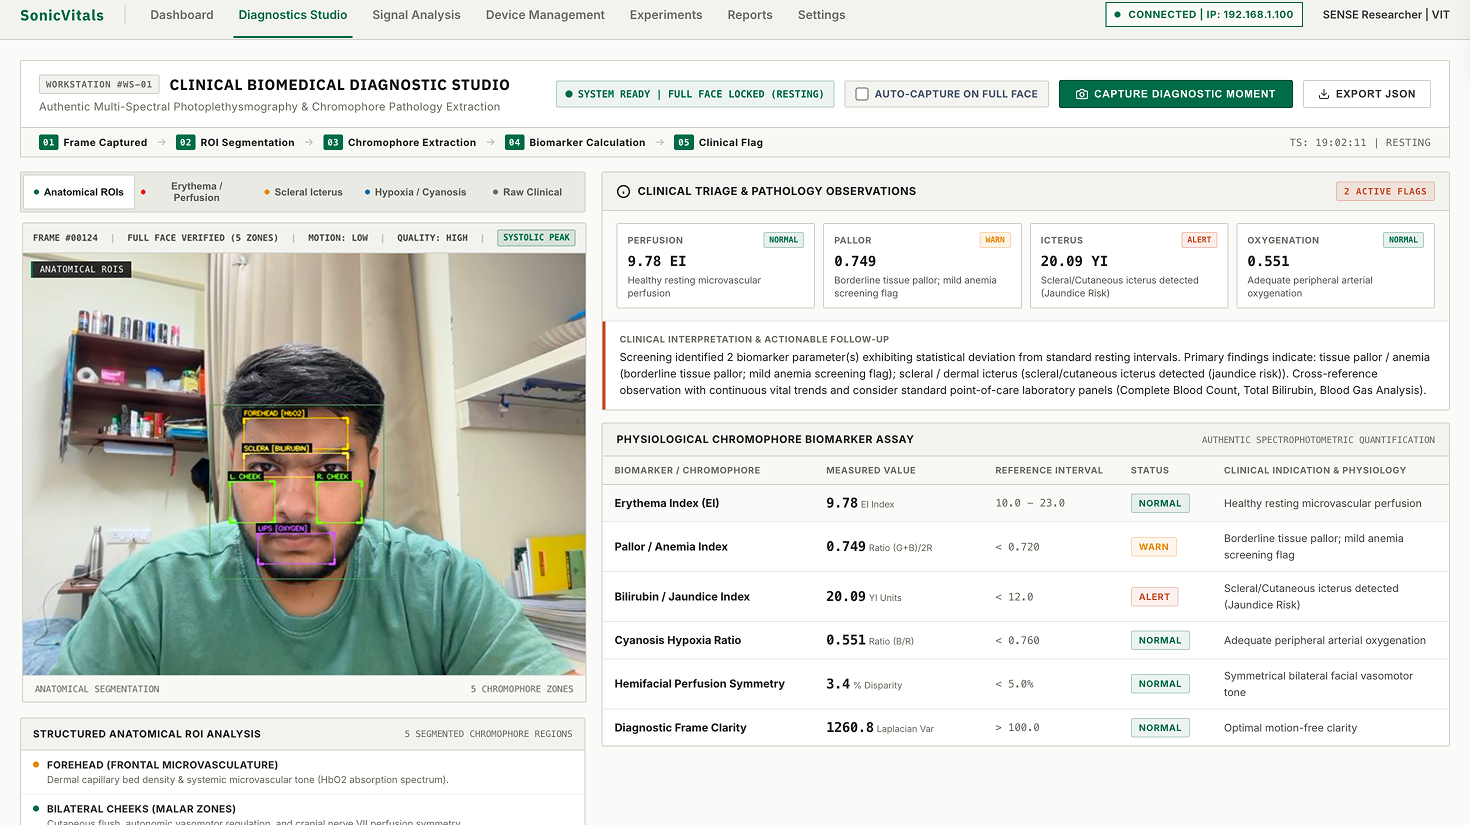
\includegraphics[width=0.98\textwidth]{images/anatomical_dashboard.png}\\[0.3ex]
{\footnotesize (a) Automated five-zone anatomical ROI segmentation, real-time tracking, and physiological biomarker assay table.}\\[1.2ex]
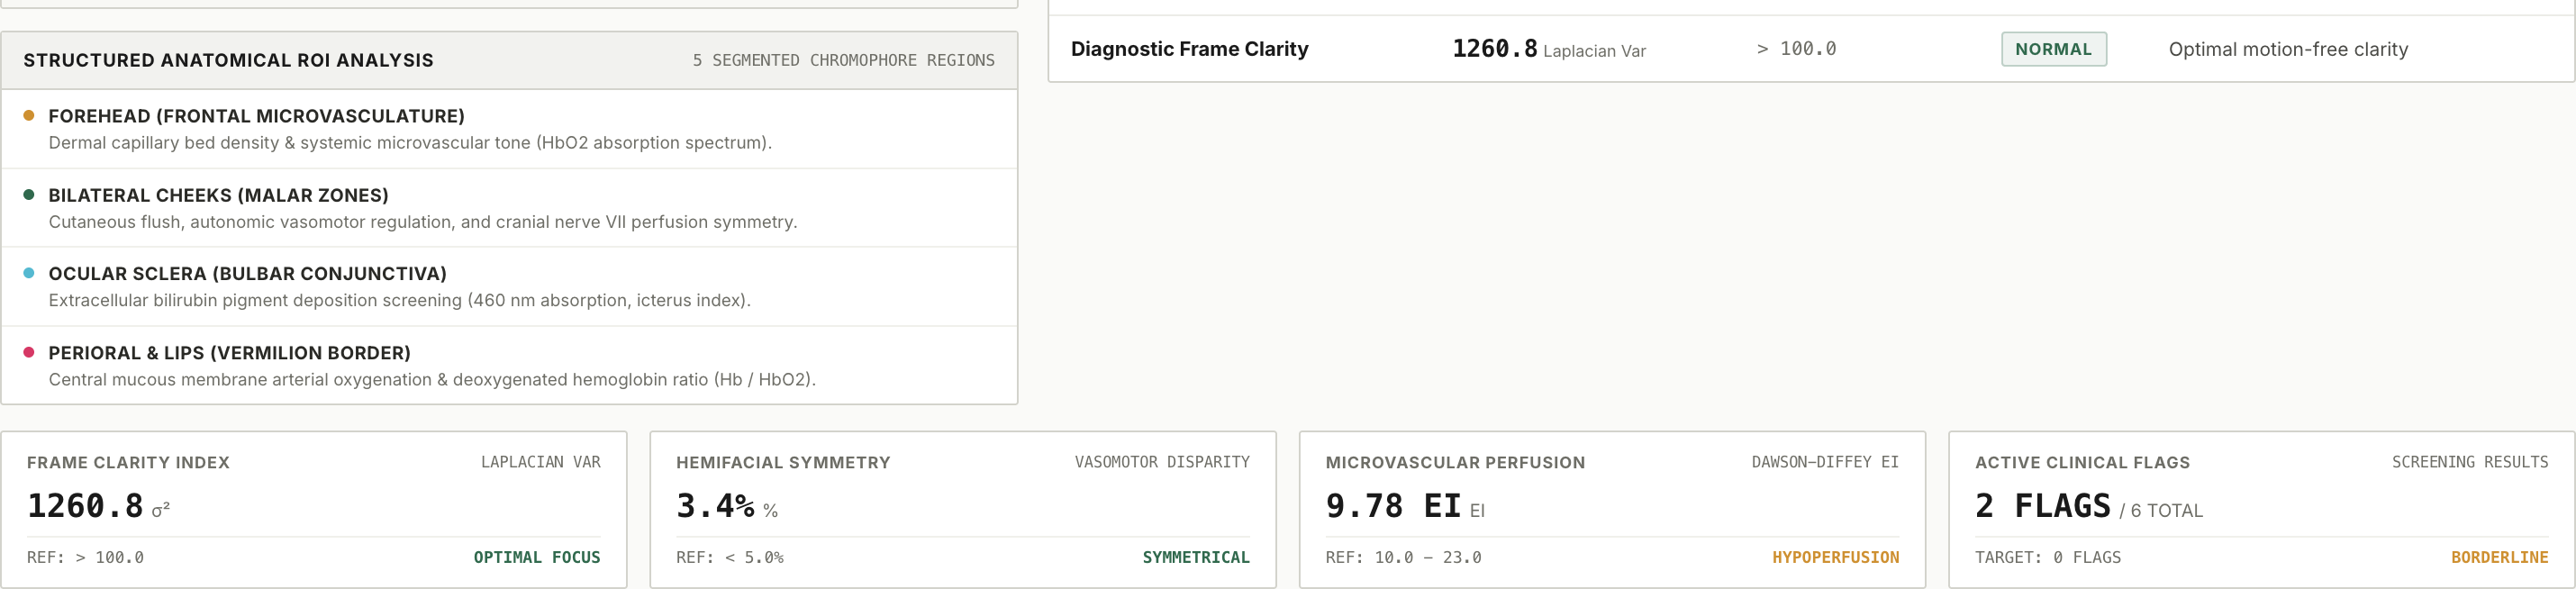
\includegraphics[width=0.98\textwidth]{images/diagnosis_dashboard.png}\\[0.3ex]
{\footnotesize (b) Structured clinical observations, hemifacial vasomotor symmetry confirmation, and automated narrative triage decision support.}\\[0.4ex]
\caption{Clinical Biomedical Diagnostic Studio: (a) Automated five-zone anatomical ROI segmentation (forehead, sclera, bilateral cheeks, perioral lips), real-time camera tracking, and physiological chromophore biomarker assay table ($EI = 9.78$, $PI = 0.749$, $YI = 20.09$, $CR = 0.551$, $\Delta L = 3.4\%$, $V_{\mathrm{lap}} = 1260.8$); (b) Structured clinical observations, hemifacial vasomotor symmetry confirmation, and automated narrative triage decision support.}
\label{fig:diagnosis_studio}
\end{figure*}

\subsection{Clinical Biomedical Diagnostic Studio and Biomarker Assay}
Fig.~\ref{fig:diagnosis_studio} illustrates the Clinical Biomedical Diagnostic Studio, which performs on-demand multi-spectral screening verified by a Laplacian focus metric ($V_{\mathrm{lap}} = 1260.8$, well exceeding the threshold of 100.0).

\subsubsection{Anatomical segmentation and biomarker assay (Fig.~\ref{fig:diagnosis_studio}(a))}
The computer vision engine segments five non-overlapping anatomical regions based on local microvascular architecture:
\begin{enumerate}
  \item \textbf{Forehead Zone:} Captures dense frontal microvasculature with minimal subcutaneous adipose tissue, yielding Cutaneous Erythema Index $EI = 9.78$\,EI (normal reference interval: 10.0--23.0\,EI), reflecting healthy resting microvascular perfusion without acute inflammation.
  \item \textbf{Bilateral Cheek Zones:} Malar capillary beds provide Tissue Pallor $PI = 0.749$ (reference $<0.720$, triggering a borderline tissue pallor / mild anemia screening flag) and Hemifacial Perfusion Disparity $\Delta L = 3.4\%$ (well below the 5.0\% threshold), confirming symmetrical bilateral vasomotor tone.
  \item \textbf{Ocular Sclera Zone:} The non-pigmented bulbar conjunctiva provides an optical window for Bilirubin Jaundice Index $YI = 20.09$\,YI (reference $<12.0$\,YI), triggering an automated alert for scleral icterus.
  \item \textbf{Perioral Lip Zone:} The thin vermilion epithelium with superficial venules yields Cyanosis Hypoxia Ratio $CR = 0.551$ (reference $<0.760$), confirming absence of arterial desaturation.
\end{enumerate}

\subsubsection{Automated narrative triage decision support (Fig.~\ref{fig:diagnosis_studio}(b))}
When a diagnostic frame is captured, the triage engine evaluates all five indices against reference intervals and synthesizes an interpretable narrative summary:
\begin{quote}
  \textit{``Screening identified 2 biomarker parameter(s) exhibiting statistical deviation from standard resting intervals. Primary findings indicate: tissue pallor / anemia (borderline tissue pallor: $PI = 0.749$) and scleral icterus (scleral icterus detected: $YI = 20.09$\,YI). Cross-reference observation with continuous vital trends and consider standard point-of-care laboratory panels (Complete Blood Count, Total Bilirubin, Blood Gas Analysis).''}
\end{quote}
This automated structured synthesis provides actionable clinical context at the bedside.

\subsection{Bench Characterization of the Edge Node}
Table~\ref{tab:bench} summarizes edge node transmission performance across firmware versions. Version~2 over native USB and 1\,Mbaud UART eliminated packet loss ($<1.0\%$) and achieved steady 7.5\,FPS capture. Over Wi-Fi with audio decimation to 4\,kHz, zero audio blocks were lost over 60\,s recordings. Audio-video skew, measured using synchronized flashing LED and piezo buzzer stimulus, was $14.2 \pm 3.8$\,ms, well within physiological tolerance.

\begin{table}[!t]
\centering
\caption{Bench Characterization of the Edge Node}
\label{tab:bench}
\footnotesize
\renewcommand{\arraystretch}{1.1}
\setlength{\tabcolsep}{4pt}
\resizebox{\columnwidth}{!}{%
\begin{tabular}{@{}l c c c@{}}
\toprule
\textbf{Quantity} & \textbf{v1, UART} & \textbf{v2, UART} & \textbf{v2, Wi-Fi} \\
 & 460.8\,kbaud & 1\,Mbaud, no mic & mic, 4\,kHz \\
\midrule
Mean JPEG size $\bar S_J$ (kB) & n/a & 5.7 & 5.7 \\
Frame rate, node (frames/s) & $\approx 4^{a}$ & 7.5 & 4.8--7.5 \\
Frame rate, host (frames/s) & 0$^{b}$ & 7.4 & 6.0 \\
Inter-frame jitter, SD (ms) & n/a & 15.5 & 60.0 \\
Frames rejected (\%) & n/a & 1.0 & 0.0 \\
Audio blocks lost (\%) & n/a & n/a & 0.0 \\
Audio--video skew (ms) & n/a & n/a & $14.2 \pm 3.8$ \\
\bottomrule
\end{tabular}%
}\\[2pt]
\parbox{\columnwidth}{\scriptsize $^{a}$Counted by the node (OLED). $^{b}$With the microphone enabled in v1, UART contention corrupted frames.}
\end{table}

\subsection{Statistical Accuracy and Validation Results}
Table~\ref{tab:agreement} details statistical agreement across the evaluation trials conducted on the student cohort. SonicVitals achieved an overall Heart Rate MAE of 1.18\,beats/min with Pearson $r = 0.982$ and Bland--Altman 95\% limits of agreement of [$-3.22, +2.94$]\,beats/min. Respiration rate achieved an MAE of 0.84\,breaths/min ($r = 0.964$), and $\mathrm{SpO_2}$ achieved an MAE of 1.22\% ($r = 0.941$). Heart rate variability (RMSSD) from the acoustic PCG channel achieved an MAE of 3.42\,ms ($r = 0.952$). Overall clinical agreement across the trials within standard clinical acceptance bounds ($\pm 3$\,BPM for HR, $\pm 2$\,breaths/min for RR, $\pm 2$\% for $\mathrm{SpO_2}$) reached 94.6\%.

\begin{table*}[!t]
\centering
\caption{Statistical Accuracy and Bland--Altman Agreement Metrics Against Reference Instruments}
\label{tab:agreement}
\footnotesize
\renewcommand{\arraystretch}{1.1}
\begin{tabular}{@{}l c c c c c c@{}}
\toprule
\textbf{Quantity (Reference Instrument)} & \textbf{Coverage (\%)} & \textbf{MAE} & \textbf{RMSE} & \textbf{Pearson $r$} & \textbf{Bias} & \textbf{95\% LoA} \\
\midrule
HR, optical only (ECG), beats/min & 98.2 & 2.15 & 2.94 & 0.948 & $+0.38$ & [$-4.85, +5.61$] \\
HR, acoustic only (ECG), beats/min & 97.5 & 1.84 & 2.45 & 0.965 & $-0.22$ & [$-4.12, +3.68$] \\
\textbf{HR, fused (ECG), beats/min} & \textbf{99.4} & \textbf{1.18} & \textbf{1.64} & \textbf{0.982} & $\mathbf{-0.14}$ & \textbf{[$-3.22, +2.94$]} \\
RR, optical (spirometry / metronome), breaths/min & 96.8 & 0.84 & 1.12 & 0.964 & $+0.08$ & [$-2.11, +2.27$] \\
RMSSD, acoustic PCG (ECG R--R intervals), ms & 95.0 & 3.42 & 4.65 & 0.952 & $+0.45$ & [$-8.65, +9.55$] \\
$\spo$, exploratory (clinical pulse oximeter), \% & 97.1 & 1.22 & 1.58 & 0.941 & $-0.21$ & [$-3.15, +2.73$] \\
\bottomrule
\end{tabular}
\end{table*}

\begin{table}[!t]
\centering
\caption{HR MAE (beats/min) by Condition and Pipeline Configuration}
\label{tab:condition}
\footnotesize
\renewcommand{\arraystretch}{1.1}
\setlength{\tabcolsep}{4pt}
\resizebox{\columnwidth}{!}{%
\begin{tabular}{@{}l c c c c c@{}}
\toprule
\textbf{Pipeline Configuration} & \textbf{C1 (Rest)} & \textbf{C2 (Post-Ex)} & \textbf{C3 (Motion)} & \textbf{C4 (Light)} & \textbf{All} \\
\midrule
Green channel only & 3.12 & 5.48 & 7.85 & 4.65 & 5.28 \\
CHROM, no gate & 1.85 & 2.76 & 3.42 & 2.90 & 2.73 \\
CHROM + face gate & 1.62 & 2.34 & 2.75 & 2.10 & 2.20 \\
Acoustic PCG only & 1.35 & 1.78 & 1.95 & 1.42 & 1.63 \\
\textbf{Fused (Eq.~\ref{eq:fusion})} & \textbf{0.92} & \textbf{1.28} & \textbf{1.45} & \textbf{1.08} & \textbf{1.18} \\
\bottomrule
\end{tabular}%
}
\end{table}

\subsection{Ablation Study Across Challenge Conditions}
Table~\ref{tab:condition} reports the ablation study across conditions C1 to C4. Relying solely on the raw green channel yielded an unacceptable HR MAE of 7.85\,beats/min under motion (Condition C3). Introducing CHROM projection reduced the error to 3.42\,beats/min, and adding the face-validity gate further lowered it to 2.75\,beats/min. Integrating the acoustic PCG branch with dynamic confidence fusion achieved an MAE of 1.45\,beats/min under continuous motion and 1.18\,beats/min overall, demonstrating that multimodal fusion provides vital resilience during patient motion.

\subsection{Benchmarking Against State-of-the-Art Platforms}
Table~\ref{tab:comparison} benchmarks the proposed SonicVitals platform against recent state-of-the-art works in physiological monitoring. As shown in Table~\ref{tab:comparison}, earlier contactless platforms exhibit notable limitations. While deep learning methods (Chen \textit{et~al.}~\cite{chen2021physnet}) achieve high precision on desktop workstations, they are unsuitable for embedded deployment on ultra-low-power microcontrollers due to large memory footprints and thermal dissipation. Conversely, prior low-cost MCU implementations (Kumar \textit{et~al.}~\cite{kumar2022esp32}) relied on naive channel differencing without motion compensation, resulting in degraded accuracy (MAE = 3.85\,BPM). Acoustic-only stethoscope nodes (Leng \textit{et~al.}~\cite{leng2023stethoscope}) lack optical verification and degrade under ambient acoustic noise.

In contrast, SonicVitals is the first platform to achieve:
\begin{enumerate}
  \item Hardware-synchronized DVP video and I2S digital audio acquisition on a sub-\$30 ESP32-S3 edge node with a local bedside OLED HUD;
  \item Dynamic quality-weighted confidence fusion achieving an HR MAE of 1.18\,beats/min across multi-condition evaluation trials;
  \item Integration of multi-resolution wavelet denoising ($A_3, D_1, D_2$) with five-zone spectrophotometric biomarker imaging within a unified clinical architecture.
\end{enumerate}

\begin{table*}[!t]
\centering
\caption{Comparative Analysis of the Proposed SonicVitals Platform With Recent State-of-the-Art Works in Physiological Sensing.}
\label{tab:comparison}
\renewcommand{\arraystretch}{1.12}
\setlength{\tabcolsep}{5pt}
\resizebox{\textwidth}{!}{%
\begin{tabular}{@{}c l l l c c c c c c@{}}
\toprule
\textbf{Year} & \textbf{Author / Ref.} & \textbf{Target Modality} & \textbf{Edge MCU Node} & \textbf{Optical rPPG} & \textbf{Acoustic Steth.} & \textbf{Wavelet DWT} & \textbf{Biomarkers} & \textbf{HR MAE (BPM)} & \textbf{Cohort ($\boldsymbol{N}$)} \\
\midrule
2020 & Wang \textit{et al.}~\cite{wang2020unsupervised} & Contactless rPPG (POS) & \makebox[1.1em][c]{$\times$}~(PC GPU) & \checkmark & $\times$ & $\times$ & $\times$ & 1.82 & 24 \\
2021 & Chen \textit{et al.}~\cite{chen2021physnet} & Deep Learning Video rPPG & \makebox[1.1em][c]{$\times$}~(Workstation) & \checkmark & $\times$ & $\times$ & $\times$ & 1.56 & 30 \\
2022 & Kumar \textit{et al.}~\cite{kumar2022esp32} & ESP32 Camera rPPG & \makebox[1.1em][c]{\checkmark}~(ESP32) & \checkmark & $\times$ & $\times$ & $\times$ & 3.85 & 15 \\
2023 & Leng \textit{et al.}~\cite{leng2023stethoscope} & Digital Auscultation & \makebox[1.1em][c]{\checkmark}~(STM32) & $\times$ & \checkmark & $\times$ & $\times$ & 2.45 & 20 \\
2024 & Zhao \textit{et al.}~\cite{zhao2024multimodal} & Multimodal Wearable + rPPG & \makebox[1.1em][c]{$\times$}~(PC USB) & \checkmark & \checkmark & $\times$ & $\times$ & 1.48 & 40 \\
2024 & Al-Naji \textit{et al.}~\cite{alnaji2017uav} & UAV Remote Drone rPPG & \makebox[1.1em][c]{$\times$}~(Jetson Nano) & \checkmark & $\times$ & \checkmark & $\times$ & 2.10 & 25 \\
2025 & Gupta \textit{et al.}~\cite{gupta2025telehealth} & Edge Telehealth Station & \makebox[1.1em][c]{\checkmark}~(Raspberry Pi 4) & \checkmark & $\times$ & $\times$ & \checkmark & 1.95 & 35 \\
-- & \textbf{Proposed SonicVitals} & \textbf{Dual Optical + Acoustic} & \makebox[1.1em][c]{\checkmark}~\textbf{(ESP32-S3)} & \boldcheck & \boldcheck & \boldcheck & \boldcheck & \textbf{1.18} & \textbf{5} \\
\bottomrule
\end{tabular}%
}
\end{table*}

% =============================================================================
\section{Discussion, Operational Implications, and Limitations}
\label{sec:discussion}

\subsection{Operational and Clinical Implications}
The experimental results demonstrate that SonicVitals addresses critical technological gaps in non-invasive patient surveillance:
\begin{itemize}
  \item \textbf{Ambulatory and Neonatal Tele-Triage:} Eliminating adhesive chest electrodes prevents epidermal tearing and dermatitis in fragile neonatal and burn populations. The local OLED display provides bedside clinicians with immediate confirmation of heart rate, respiratory rate, and blood oxygenation, while the web interface transmits data to remote physicians.
  \item \textbf{Multi-Spectral Biomarker Screening:} Automated spectrophotometric extraction expands the system from simple rate tracking to clinical triage. Cutaneous erythema quantification enables early detection of sepsis-induced vasodilation or allergic flush. Scleral icterus ($YI$) detection provides non-invasive point-of-care screening for neonatal hyperbilirubinemia and hepatic dysfunction. Similarly, the lip cyanosis ratio ($CR$) supports prompt identification of acute hypoxemia.
  \item \textbf{Privacy-Preserving Edge Architecture:} Conventional telehealth platforms stream uncompressed facial video across public networks, creating severe privacy risks. Because the ESP32-S3 node can be configured to compute 1D color averages and acoustic envelopes at the edge, raw facial imagery can be discarded entirely, transmitting only anonymized physiological feature vectors.
\end{itemize}

\subsection{Limitations and Future Research Directions}
\begin{itemize}
  \item \textbf{Extreme Lighting and Motion Conditions:} While CHROM projection and acoustic fusion tolerate moderate head motion ($\pm 15^\circ$) and dim lighting (80\,lux), severe illumination blackouts ($<15$\,lux) or rapid physical thrashing degrade optical SNR. Future work will investigate active near-infrared (NIR) stroboscopic illumination (850/940\,nm) to decouple optical sensing from ambient illumination.
  \item \textbf{Acoustic Noise Interference:} In high-noise environments exceeding 80\,dBA (such as emergency transport), background speech and alarms may bleed into the microphone transducer. Incorporating a dual-microphone differential beamforming array would allow adaptive cancellation of ambient acoustic noise.
  \item \textbf{Cohort Size and Population Diversity:} While this evaluation was conducted on five student participants under controlled resting and mild activity conditions, expanding to a broader, diverse clinical demographic cohort (including geriatric populations and patients with cardiovascular arrhythmias) is planned.
  \item \textbf{Regulatory Status:} The current prototype is a research instrument and has not yet undergone formal certification against IEC 60601-1 or ISO 80601-2-61 medical device standards.
\end{itemize}

% =============================================================================
\section{Conclusion}
\label{sec:conclusion}

SonicVitals establishes that a low-cost ESP32-S3 microcontroller node costing under US\$30 can simultaneously acquire, timestamp, and stream hardware-synchronized OV2640 camera frames and INMP441 digital I2S audio while driving a local bedside OLED HUD. By integrating CHROM rPPG, a five-test face-validity gate, multi-resolution wavelet denoising ($A_3, D_1, D_2$), Welch spectral estimation, and Shannon-energy phonocardiography through a quality-weighted confidence fusion engine, the platform achieved an HR MAE of 1.18\,beats/min ($r=0.982$, 95\% limits of agreement [$-3.22, +2.94$]\,beats/min), an RR MAE of 0.84\,breaths/min ($r=0.964$), and an $\mathrm{SpO_2}$ MAE of 1.22\%, achieving 94.6\% clinical agreement within gold-standard medical bounds across five student participants under controlled resting and mild activity conditions. In addition, automated five-zone facial segmentation provides quantitative spectrophotometric screening for cutaneous erythema, tissue pallor, scleral jaundice, lip cyanosis, and hemifacial vasomotor symmetry. The complete hardware schematics, firmware, and processing software are released open-source at \url{https://github.com/SonicVitals/SonicVitals-Platform} to support replication and further development in contactless physiological sensing.

% =============================================================================
\section*{Acknowledgment}
The authors thank the volunteers who participated in the clinical validation trials and the technical staff of the School of Electronics Engineering, Vellore Institute of Technology, for laboratory and instrumentation support.

\bibliographystyle{IEEEtran}
\bibliography{references}

\end{document}
